\chapter{Recursive Data Interpolation Techniques} % Neural decoder
\chaptermark{Interpolation}
%\thispagestyle{empty}
\label{sec:data interpolation}



Ch.~\ref{sec:copulas} described how, from $N$ data points $(x_1,\dots, x_N)$, it is possible to leverage NNs to interpolate a function representing the underlying PDF $p_X(x)$ that generated the observed data. In all the previous contexts, interpolation effectively meant estimating the distribution of the given samples in order to understand the \textit{stochastic} nature of the data. We typically exploit $p_X(x)$ to produce new realizations $(\hat{x}_1,\dots, \hat{x}_N)$.

In this chapter, instead, we focus on capturing the \textit{deterministic} relationship between inputs and outputs, determining a function that passes through specific points. 
When we approach interpolation from the perspective of finding a fitting function, we aim to create a mathematical model that accurately represents the relationship between the given data points, abstracting from how these points have been obtained. 
This fitting function allows us to predict intermediate values within the range of the data, enabling smooth transitions between observed points.

Fitting functions are extremely useful for trajectory generation in various fields such as physics, robotics and aerospace engineering. When designing trajectories for moving objects or systems, it is essential to create smooth and continuous paths that meet specific constraints and objectives.
In the following, we study the trajectory generation problem and propose a novel iterative interpolation technique.

The results presented in this chapter are documented in \cite{Letizia2020_rst, LetiziaRobotics, 9525383}.

\label{sec:rst}
% 
% 
The widespread integration of communication networks and smart devices in modern control systems has increased the vulnerability of industrial systems to online cyber-attacks, e.g., Industroyer, Blackenergy, etc \citep{osti_1505628}.
% Modern control systems have seen a large push to include communication networks and smart devices to increase performance, made possible by improvements in communication device cost and energy consumption. This trend has been coupled with the usage of open-standard communication protocols among industrial control systems, making them vulnerable to online cyber-attacks such as Industroyer, Blackenergy, etc \citep{osti_1505628}. 
To counter this, methods have been developed to improve security by achieving attack detection, mitigation, and monitoring, among others \citep{sandberg2022secure}. This paper focuses on active attack diagnosis to mitigate stealthy attacks. 
%
%\subsection{Literature review}

Active diagnosis techniques rely on the inclusion of additional moduli to control systems
% inclusion within the control system of additional moduli 
to alter the behavior of the system compared to information known by the attacker. 
For instance, the concept of additive watermarking was introduced in \cite{mo2015physical}, where noise signals of known mean and variance are added at the plant and compensated for it at the controller. 
This compensation, however, is not exact, causing some performance degradation. Thus, trade-offs between performance and detectability  are necessary \citep{zhu2023detection}.
% A later work \citep{zhu2023detection} designs the watermark signal by trading performance for detection. Thus, although additive watermarking serves as a good detection scheme, they endure performance losses even in the nominal case. 

In encrypted control \citep{darup2021encrypted}, the sensor data is encrypted, sent to the controller, and then operated on directly. Encrypted input signals are sent back to the plant for decryption. Although encryption is widespread in IT security, in control systems it presents some concerns, such as the introduction of time delays \citep{stabile2024verifiable}, while it may present inherent weaknesses \citep{alisic2023model}.
% they are not preferred as they introduce time delays \citep{stabile2024verifiable} which can cause instability, and some encryption schemes can be very weak  \citep{alisic2023model}. 

In moving target defense \citep{griffioen2020moving}, the plant is augmented with fictitious dynamics, known to the controller. The plant output is transmitted to the controller along with the fictitious states over a network under attack. 
The additional measurements then aide in the detection of attacks. 
This comes at the cost of higher communication bandwidth needs, which increases rapidly with the dimension of the augmented systems.
% Since the dynamics of the fictitious dynamics are exactly known to the controller, the attack is detected easily. However, when the scale of the system increases, the communication bandwidth used by moving the target defense approach increases rapidly. 

Other recently proposed works include two-way coding \citep{fang2019two}, a weak encryuption technique, and dynamic masking \citep{abdalmoaty2023privacy}, which enhances privacy as well as security, have been shown to be effective against zero-dynamics attacks.
% Two-way coding \citep{fang2019two} and dynamic masking \citep{abdalmoaty2023privacy} are other recently proposed approaches. Two-way coding is another form of weak encryption technique whilst dynamic masking proposes an architecture that enhances both privacy and security. These schemes are shown to be effective against zero dynamics attacks but remain to be studied for other classes of attacks. 
% Recent extensions include \citep{mukherjee2021secure,ramos2024privacy}.
% Some other works which are related are \citep{mukherjee2021secure}, an extension of \cite{fang2019two}. The work \citep{ramos2024privacy} is an extension of moving target defense for multi-agent systems. 
Furthermore, filtering techniques for attack detection are proposed by \cite{murguia2020security,hashemi2022codesign,escudero2023safety}, while not focusing on stealthy attacks.
% The works \citep{murguia2020security,hashemi2022codesign,escudero2023safety} develop filtering techniques to guarantee safety, without being focused on stealthy covert attacks.

Multiplicative watermarking (mWM) has been proposed by the authors as a diagnosis technique \citep{ferrari2020switching}. mWM consists of a pair of filters on each communication channel between the plant and its controller; the scheme is affine to weak encryption, whereby ``encoding'' and ``decoding'' are done by changing signals' dynamic characteristics through inverse pairs of filters. This enables original signals to be recovered exactly, and thus does not lead to performance degradation.
% A multiplicative watermark is an affine to a weak encryption technique, through which the signal is ``encoded'' by a filter, changing its dynamic behavior. The use of inverse pairs means that the original signal can be recovered, through ``decoding'' via an inverse filter. As such, differently to techniques based on additive watermarking, no performance is lost due to the injection of noise, and there are no bandwidth limitations.

%\subsection{Contributions}
One of the critical features of multiplicative watermarking is that to detect stealthy attacks, the mWM filter parameters must be switched over time. In this paper, an algorithm to optimally design the mWM parameters after a switching event is presented, enhancing detection performance, without changing the switching time.
% This is done without changing the switching time, which is taken as given.

\textcolor{black}{
To formalize the filter design problem, we suppose the defender is interested in optimal performance against adversaries injecting covert attacks with matched system parameters \citep{smith2015covert}, including the mWM parameters prior to the switch. This scenario represents a worst case where malicious agents can take full control of the system while remaining undetected.
Thus, the attack strategy is explicitly included within the formulation of the closed-loop system, and the mWM filters are chosen by solving an optimization problem minimizing the attack-energy-constrained output-to-output gain (AEC-OOG) \citep{anand2023risk}, a variation of the output-to-output gain proposed in  \cite{teixeira2015strategic}.
}
The main contributions of this paper are:
% We consider an adversary injecting a covert attack with matched system parameters \citep{smith2015covert}, i.e., an attacker with full knowledge of the control system parameters, including those of the mWM filters before the switch. This scenario is taken as a worst case, as it has been shown that this class of attacks can be made stealthy. To quantitatively define a cost, the output-to-output gain (OOG) \citep{teixeira2015strategic} is leveraged,
% a metric introduced to evaluate the impact of an additive attack in a control system. %Specifically, OOG evaluates the worst-case performance loss that an attacker injecting an undetectable attack can obtain. 
% Here, the maximum performance loss caused by a stealthy adversary with limited energy is taken, the attack-energy-constrained OOG (AEC-OOG) \citep{anand2023risk}. The main contributions of this paper are:
\begin{enumerate}
%[label=\alph*.]
\item The problem of optimally designing the switching mWM filters is formulated as an optimization problem, with the AEC-OOG is taken as the objective;%where the AEC-OOG is taken as the impact metric; 
\item The worst-case scenario of a covert attack with exact knowledge of plant and mWM filter parameters is embedded within the design problem;
% The optimization problem is defined to incorporate the worst-case scenario of a covert attack with exact knowledge of plant and mWM filter parameters;
\item The feasibility of the optimization problem is shown to be dependent only on stability conditions; 
\item A solution scheme is proposed to promote randomization of the mWM filter parameters such that an eavesdropping adversary cannot remain stealthy.
\end{enumerate} 

This builds on the results of \cite{ferrari2020switching}, where the focus was on the design of the switching protocols, rather than the parameters themselves.
Compared to previous work \citep{gallo2021design}, this paper introduces an optimization problem which is always feasible (thanks to the use of AEC-OOG in the objective), while also considering a more sophisticated class of covert attacks, where the presence of watermark is known to the adversary. 
Moreover, this paper poses a different objective than \citep{zhang2023hybrid}; indeed, while \citep{zhang2023hybrid} provided a design strategy to ensure certain privacy properties, in this paper we address the problem of optimal parameter design following a switching event.


%\subsection{Organization}
The rest of the paper is organized as follows. 
After formulating the problem in Section~\ref{sec:PF}, we propose our design algorithm in Section~\ref{sec:main}, and analyze its properties. It is then evaluated through a numerical example in Section~\ref{sec:NE}, and concluding remarks are given Section~\ref{sec:Con}.
% We provide the problem background in Section~\ref{sec:PF}. We formulate the design problem in Section~\ref{sec:main}, together with an analysis of its properties. The proposed algorithm is evaluated through a numerical example in Section \ref{sec:NE}. Concluding remarks are offered in Section \ref{sec:Con}.
\section{Problem statement}
\label{subsec:rst_problem}
Consider the problem of navigating a moving body, e.g., an unmanned vehicle, through $N+1$ waypoints at specific time stamps. Assume that any arbitrary dynamic limitation of the  body translates into kinematic constraints (e.g. position, velocity, acceleration, etc.). Such kinematic constraints are useful to impose, for instance, that the body starts from the rest at the beginning of the trajectory and reaches each waypoint with specific kinematics (e.g. aggressive maneuvering).

The task of path planning consists of finding a trajectory $\mathbf{x}(t)$ to move a given body from an initial point $\mathbf{x}(t_0)$ to a final point $\mathbf{x}(t_N)$, minimizing a certain cost function $J(\cdot)$ (time, energy, jerk, etc.), under given geometrical and kinematic constraints $\sigma(\cdot)$.

Let $t_0<t_1<\dots<t_N$ be $N+1$ time stamps for which all the corresponding positions $\mathbf{x}(t_0),\mathbf{x}(t_1), \dots, \mathbf{x}(t_N)$ and the respective $k$ derivatives $\frac{d^i\mathbf{x}}{dt^i}\bigr|_{t=t_0}, \frac{d^i\mathbf{x}}{dt^i}\bigr|_{t=t_1}, \dots, \frac{d^i\mathbf{x}}{dt^i}\bigr|_{t=t_N}$ are a-priori assigned, for $i = 1,\dots, k$. For notation convenience, the trajectory for which the first $k$ derivatives are defined, is denoted with $\mathbf{x}_k(t)$.

The objective is to design a feasible trajectory $\mathbf{x}_k(t)$ which satisfies the equality kinematic constraints $\sigma_{i,j}$ expressed by the first $k$ derivatives $\frac{d^i\mathbf{x}}{dt^i}\bigr|_{t=t_j} = \sigma_{i,j} $, for $i=0,1,\dots,k$ and $j=0,1,\dots,N$. 

To do so we propose to use polynomials as the set of our feasible trajectories. In particular, we build the polynomial trajectory as a linear combination of $k+1$ polynomial basis
\begin{equation}
\label{eq:rst_trajectory}
\mathbf{x}_k(t) = \sum_{i=0}^{k}{\mathbf{p}_i(t)},
\end{equation}
where $\mathbf{p}_i(t)$ is the polynomial (for each component of the $3D$ space) \textit{responsible} for the fulfillment of the $i$-th derivative constraint and $k$ is the number of considered derivatives. In other words, each polynomial component $\mathbf{p}_i(t)$ is designed as an additive term which iteratively fulfills the $i$-th kinematic constraint.
Furthermore, we exploit Lagrange interpolating polynomials to compute the polynomial basis $\mathbf{p}_i(t)$.

To the best of authors' knowledge, this is the first work that recursively builds a set of polynomials for trajectory generation under kinematic constraints.






\section{Theoretical formulation of RST}
\label{subsec:rst_results}
This section presents the mathematical foundations behind the choice of the polynomial representation in \eqref{eq:rst_trajectory}. We show that such choice produces a closed form continuous polynomial trajectory and enables an iterative algorithm for its generation. In particular, Lagrange polynomials are exploited. For ease of notation, in the following we consider the trajectory in \eqref{eq:rst_trajectory} as unidimensional, assuming that the $3D$ extension is obtained by working component-wise.%
\subsection{Preliminaries on Lagrange polynomials}
\label{subsec:rst_Lagrange}
Lagrange polynomials offer a technique to interpolation problems. In particular, given a set of $N+1$ $1D$ control points (waypoints) $(t_0,x(t_0)), (t_1,x(t_1)), \dots, (t_N,x(t_N))$, the interpolation polynomial in the Lagrange form is defined as
\begin{equation}
\label{eq:rst_lagrange}
L(t) := \sum_{j=0}^{N}{x(t_j) \ell_j(t)}
\end{equation}
where $\ell_j(t)$ is the Lagrange polynomial basis whose form reads as follows
\begin{equation}
\ell_j(t):= \prod_{\substack{m=0 \\ m\neq j}}^{N}{\frac{t-t_m}{t_j-t_m}},
\end{equation}
with $0\leq j\leq N$. The main idea behind this definition is that, by construction, the $N+1$ basis functions are such that $\ell_j(t_i)\equiv 0$ in $i=0,\dots,N \; \wedge \; i\neq j$. So for each waypoint, only one single basis function contributes to the sum in \eqref{eq:rst_lagrange}.

\subsection{The recursive formula}
To discover the recursive property behind the formulation in \eqref{eq:rst_trajectory}, we start the mathematical derivation introducing two lemmas regarding a particular polynomial choice and its derivatives. Such type of choice enables a remarkable recursive property which is proved in Theorem \ref{theorem:rst_theorem1}, the main result of this chapter. The corollary \ref{corollary:rst_corollary1}, instead, establishes an upper bound for the minimum degree of the polynomial trajectory generated via the recursive formulation.

\begin{lemma}
\label{lemma:rst_Lemma1}
Let
\begin{equation}
a(t) = \prod_{n=0}^{N}{(t-t_n)},
\label{eq:rst_a_t}
\end{equation}
then
\begin{equation}
\frac{d}{dt}a(t) = a(t)\cdot \sum_{n=0}^{N}{\frac{1}{t-t_n}}
\label{eq:rst_da_t}
\end{equation}
and
\begin{equation}
\frac{d}{dt}a(t)\biggr|_{t=t_j} = \prod_{\substack{n=0\\ n\neq j}}^{N}{(t_j-t_n)}.
\label{eq:rst_da_tj}
\end{equation}
\end{lemma}
\begin{proof}
Using product rule
\begin{equation}
\frac{d}{dt}a(t) = \sum_{j=0}^{N}{\prod_{\substack{n=0\\ n\neq j}}^{N}{(t-t_n)}}.
\label{eq:rst_Lemma1}
\end{equation}
Dividing and multiplying by $a(t)$ gives \eqref{eq:rst_da_t}. For $t=t_j$ only one term of the summation in \eqref{eq:rst_Lemma1} contributes leading to \eqref{eq:rst_da_tj}. \qedhere  
\end{proof}

\begin{lemma}
\label{lemma:rst_Lemma2}
Let
\begin{equation*}
a(t) = \prod_{n=0}^{N}{(t-t_n)},
\end{equation*}
and let $s(t)$ be a polynomial. Then
\begin{equation}
\frac{d^h}{dt^h}\biggl[\frac{a^k(t)}{k!}\cdot s(t)\biggr]_{t=t_j} \equiv 0 \; \forall k>h
\label{eq:rst_diff_ak}
\end{equation}
and
\begin{equation}
\frac{d^h}{dt^h}\biggl[\frac{a^h(t)}{h!}\cdot s(t)\biggr]_{t=t_j} = \biggl(\frac{d}{dt}a(t)\biggr)^h\ \biggr|_{t=t_j} \cdot s(t_j).
\label{eq:rst_diff_ah}
\end{equation}
\end{lemma}
\begin{proof}
Since $t=t_j$ is a zero of $a^k(t)$ with multiplicity $k>h$, the factor $(t-t_j)$ appears in every term of the $h$-th derivative. If $k=h$, then
\begin{equation}
\frac{d^h}{dt^h}\biggl[\frac{a^h(t)}{h!}\cdot s(t)\biggr]_{t=t_j} = \frac{d^{h-1}}{dt^{h-1}}\biggl[\frac{d}{dt} \biggl(\frac{a^h(t)}{h!}\cdot s(t)\biggr)\biggr]_{t=t_j}.
\end{equation}
By the linearity of the differential operator and product rule, RHS can be rewritten as
\begin{equation}
\frac{d^{h-1}}{dt^{h-1}}\biggl[\frac{a^{h-1}(t)}{{h-1}!}\cdot \frac{d a(t)}{dt}\cdot s(t)\biggr]_{t=t_j} + \cancel{\frac{d^{h-1}}{dt^{h-1}}\biggl[\frac{a^h(t)}{h!}\cdot \frac{d}{dt}s(t)}\biggr]_{t=t_j}
\end{equation}
where the second term in the above expression vanishes because of the first part of the lemma. Proceeding in the same way until the $h$-th derivative leads to
\begin{equation}
\frac{d^h}{dt^h}\biggl[\frac{a^h(t)}{h!}\cdot s(t)\biggr]_{t=t_j} = \biggl(\frac{d}{dt}a(t)\biggr)^h\ \biggr|_{t=t_j} \cdot s(t_j)
%\label{eq:rst_diff_ah}
\end{equation}
which concludes the proof. \qedhere  
\end{proof}

To understand the terms involved while building the final trajectory $x_k(t)$, the concept of $m$-partial trajectory is introduced.
\begin{defn}
\label{def:rst_def1}
Let $\frac{d^i}{dt^i}x_k(t)\bigr|_{t=t_j}$ be given kinematic constraints, for $i=0,1,\dots, k$. An $m$-partial trajectory is a feasible trajectory which only fulfills the first $m$ kinematic constraints, i.e. 
\begin{equation}
x_m(t) = \sum_{i=0}^{m}{p_i(t)}, \; \text{with }\; m\leq k.
\end{equation} 
\end{defn}
As an example, if the kinematic constraints are set up to the acceleration ($k=2$), a $1$-partial trajectory is a polynomial trajectory that passes through the $N+1$ waypoints with the given velocities.

\begin{theorem}
\label{theorem:rst_theorem1}
Let $t_j$ be a point in time, for $j=0,1,\dots, N$, such that $\frac{d^i}{dt^i}x_k(t)\bigr|_{t=t_j}=\sigma_{i,j}$ is the associated given kinematic constraint, for $i=0,1,\dots, k$. Let $x_k(t)$ be a feasible polynomial trajectory defined as
\begin{equation}
x_k(t) = \sum_{i=0}^{k}{p_i(t)}.
\end{equation}
If
\begin{equation}
p_i(t)=\dfrac{1}{i!}\biggl(\prod_{n=0}^{N}{(t-t_n)}\biggr)^i\cdot s_i(t)
\end{equation}
then the $i$-partial trajectory $x_i(t)$ depends recursively on $x_{i-1}(t)$. In particular,
\begin{equation}
s_i(t_j)=\dfrac{\dfrac{d^i}{dt^i}x_k(t)\biggr|_{t=t_j} -\dfrac{d^i}{dt^i}x_{i-1}(t)\biggr|_{t=t_j}}{\displaystyle \Biggl(\prod_{\substack{n=0\\ n\neq j}}^{N}{(t_j-t_n)}\Biggr)^i}.
\label{eq:rst_recursive}
\end{equation}
\end{theorem}

\begin{proof}
For $i=0$, $x_{-1}(t):=0$ and the kinematic constraint is $x_k(t_j)$ which brings to the first polynomial $s_0(t)=p_0(t)=x_0(t)$ obtained using an interpolation technique, e.g. the Lagrange polynomials as explained in Sec. \ref{subsec:rst_Lagrange}. No other contributions $p_i(t)$ are taken into account since $p_i(t_j)=0 \; \forall i>0$. For brevity of notation it is now convenient to define a polynomial $a(t)$ as $a(t) = \prod_{n=0}^{N}{(t-t_n)}$.

For $i=1$ and constraint $\frac{d}{dt}x_k(t)\bigr|_{t=t_j}$, 
\begin{equation}
x_k(t) = x_0(t) + a(t)\cdot s_1(t) + \sum_{i=2}^{k}{\dfrac{a^i(t)}{i!}s_i(t)},
\label{eq:rst_i1}
\end{equation}
taking the derivative in $t_j$ in both sides of \eqref{eq:rst_i1} yields to
\begin{equation}
\frac{d}{dt}x_k(t)\biggr|_{t=t_j} = \frac{d}{dt}x_0(t)\biggr|_{t=t_j} + \frac{d}{dt}a(t)\biggr|_{t=t_j}\cdot s_1(t_j)
\end{equation}
where, using Lemma \ref{lemma:rst_Lemma2}, no contribution in $t_j$ comes from $i>1$. Rearranging,
\begin{equation}
s_1(t_j)=\dfrac{\dfrac{d}{dt}x_k(t)\biggr|_{t=t_j} -\dfrac{d}{dt}x_0(t)\biggr|_{t=t_j}}{\displaystyle \prod_{\substack{n=0\\ n\neq j}}^{N}{(t_j-t_n)}}
\end{equation}
where the denominator is a consequence of Lemma \ref{lemma:rst_Lemma1}.
To compute $s_1(t)$, it is convenient to interpolate the points $s_1(t_j)$ again with Lagrange polynomials. The $1$-partial trajectory has expression $x_1(t)=x_0(t)+a(t)\cdot s_1(t)$.

In general, for $i=h$ the constraint to be fulfilled is $\frac{d^h}{dt^h}x_k(t)\bigr|_{t=t_j}$. Thus
\begin{equation}
x_k(t) = x_{h-1}(t) + \dfrac{a^h(t)}{h!}\cdot s_h(t) + \sum_{i=h+1}^{k}{\dfrac{a^i(t)}{i!}\cdot s_i(t)},
\label{eq:rst_ih}
\end{equation}
where $x_{h-1}(t)$ is the $(h-1)$-partial trajectory. Taking the $h$-th derivative in $t_j$ in both sides of \eqref{eq:rst_ih} and using again Lemma \ref{lemma:rst_Lemma2} for the second and third term, yields to
\begin{equation}
\frac{d^h}{dt^h}x_k(t)\biggr|_{t=t_j} = \frac{d^h}{dt^h}x_{h-1}(t)\biggr|_{t=t_j} + \biggl(\frac{d}{dt}a(t)\biggr)^h\ \biggr|_{t=t_j} \cdot s_h(t_j).
\end{equation}
Finally, rearranging
\begin{equation}
s_h(t_j)=\dfrac{\dfrac{d^h}{dt^h}x_k(t)\biggr|_{t=t_j} -\dfrac{d^h}{dt^h}x_{h-1}(t)\biggr|_{t=t_j}}{\displaystyle \Biggl(\prod_{\substack{n=0\\ n\neq j}}^{N}{(t_j-t_n)}\Biggr)^h}
\end{equation}
concludes the proof. \\ \qedhere  
\end{proof}

Theorem \ref{theorem:rst_theorem1} provides a recursive formula to evaluate the points $s_i(t_j)$. Hence, it is sufficient to interpolate them, for example with Lagrange polynomials, in order to get $s_i(t)$ at each iteration. As a remark, the interpolation of $s_i(t_j)$ can be carried out also by adopting other polynomial basis functions, e.g., Newton polynomials, B-Spline, etc. Nevertheless, the polynomial assumption comes from Lemma \ref{lemma:rst_Lemma2}. Indeed, polynomials, when differentiated, do not introduce extra poles which could cancel with $a(t)$. On the contrary, other basis functions do not guarantee this property.

The following corollary provides an information on the minimum degree of the polynomial trajectory $x_k(t)$ defined in \eqref{eq:rst_trajectory}.

\begin{corollary}
\label{corollary:rst_corollary1}
Let $t_j$ be a point in time, for $j=0,1,\dots, N$, such that $\frac{d^i}{dt^i}x_k(t)\bigr|_{t=t_j}$ is the associated given kinematic constraint, for $i=0,1,\dots, k$. If $x_k(t)$ is a feasible polynomial trajectory defined as
\begin{equation}
x_k(t) = \sum_{i=0}^{k}{\dfrac{1}{i!}\biggl(\prod_{n=0}^{N}{(t-t_n)}\biggr)^i\cdot s_i(t)},
\end{equation}
then the minimum degree of $x_k(t)$ is less or equal to $(k+1)(N+1)-1$.
\end{corollary}
\begin{proof}
Each $s_i(t)$ is a Lagrange polynomial that passes through $N+1$ points, therefore its minimum degree is $N$. The highest contribution in terms of degree to $x_k(t)$ comes when $i=k$, so that $\prod_{n=0}^{N}{(t-t_n)^k}$ is a polynomial of degree equal to $(N+1)k$. Thus, the product of $\prod_{n=0}^{N}{(t-t_n)^k}$ and $s_k(t)$ gives a polynomial whose minimum degree is at most $(N+1)k+N = (k+1)(N+1)-1$.
This is somehow consistent with the idea that imposing $k+1$ constraints for each of the points in time $t_j$ gives $(k+1)(N+1)$ constraints and the minimum degree of a polynomial that satisfies them is $(k+1)(N+1)-1$. \qedhere
\end{proof}

\subsection{Recursive smooth trajectory generation}
\label{subsec:rst_code}

\begin{figure}[t]
\includegraphics[scale=0.40]{images/extra/RST_all}
\centering
\caption{RST block diagram.}
\label{fig:rst_RST}
\end{figure}
In the following, we will denote our approach as recursive smooth trajectory (RST) generation. The idea behind it, is that each component $p_i(t)$ in \eqref{eq:rst_trajectory} guarantees that $\dfrac{d^i}{dt^i}x_k(t)\bigr|_{t=t_j}=\sigma_{i,j}$ is fulfilled. Starting from the waypoints constraint which can be easily calculated through Lagrange polynomials, all the following higher-order differential kinematic constraints depend recursively on previous ones, according to \eqref{eq:rst_recursive}. 

The pseudocode in Alg.~\ref{alg:RST} provides a practical idea on how to iteratively design the trajectory $x_k(t)$ under the conditions aforementioned. The scheme in Fig.~\ref{fig:rst_RST} illustrates how RST operates.



We now discuss the influence of the distribution of the time instants $t_j$ for $j=0,\dots,N$ over the trajectory on oscillations and numerical limitations by proposing a known solution (Chebyshev nodes) and a novel hybrid solution, denoted as blockwise recursive smooth trajectory (BRST) that tackle said practical issues.

\begin{algorithm}
\caption{Recursive smooth trajectory (RST) generation}
\label{alg:RST}
\begin{algorithmic}[1]
\Inputs{$N+1$ points in time $t_0<t_1<\dots<t_N$; \\ Number of derivatives $k$ to fulfill; \\ Kin. constr. $\frac{d^i}{dt^i}x_k(t)\bigr|_{t=t_0}, \dots, \frac{d^i}{dt^i}x_k(t)\bigr|_{t=t_N}$.}
\Initialize{$a(t)=(t-t_0)\cdots (t-t_N)$ polynomial; \\ $x_{-1}(t) \equiv 0$.}
\For{$i=0$ to $k$}
	\For{$j=0$ to $N$}
		\State $s_i(t_j)=\dfrac{\dfrac{d^i}{dt^i}x_k(t)\biggr|_{t=t_j} -\dfrac{d^i}{dt^i}x_{i-1}(t)\biggr|_{t=t_j}}{\displaystyle \Biggl(\dfrac{d}{dt}a(t)\biggr|_{t=t_j}\Biggr)^i}$;
	\EndFor
	\State Interpolate $s_i(t_j)$ with Lagrange polynomial $s_i(t)$;
	\State $x_i(t) = x_{i-1}(t)+\dfrac{a^i(t)}{i!}\cdot s_i(t)$;
\EndFor
\end{algorithmic}
\end{algorithm}

\subsection{Remarks and insights on blockwise approach}
In the previous sections, we presented the formal generation approach (RST) of $x_k(t)$ for points in time $t_0<t_1< \dots <t_N$ with no constraints on $N$ and on the length of the interval $I_j = t_{j+1}-t_j$ for $j = 0,\dots, N-1$. 
Unfortunately, when the number of points $N+1$ is large and in particular when points in time $t_j$ are equally spaced ($I_j$ is constant), the Runge's phenomenon may occur \cite{Runge}. The Runge's phenomenon is an oscillation problem near the endpoints of the polynomial interpolation function, as illustrated in Fig. \ref{fig:rst_Runge}. To overcome it, one could either move to spline interpolation as mentioned in Sec. \ref{subsec:rst_introduction} or change the distribution of the nodes $t_j$ more densely towards the edges of the interval $[t_0, t_N]$ as proposed in \cite{Berrut}.
In the latter case, a standard choice considers the set of points in time as the set of Chebyshev nodes. In particular, for $N+1$ points in the interval $[t_0, t_N]$, nodes are transformed into
\begin{equation}
\hat{t}_j = \frac{1}{2}(t_0+t_N) + \frac{1}{2}(t_N-t_0)\cos\biggl[\dfrac{2j+1}{2(N+1)}\pi\biggr], \; j = 0,\dots, N.
\label{Cheby}
\end{equation}

Moreover, when the number of points $N+1$ increases, we encounter computational limitations in evaluating the powers $t^{(k+1)(N+1)-1}$. In such a case, a possible new blockwise approach that we name blockwise RST (BRST) concatenates intervals 
\begin{equation}
    [t_{0,1},t_{N,1}], [t_{0,2},t_{N,2}], \dots, [t_{0,M},t_{N,M}]
\end{equation} 
in $M$ blocks. For each block, the associated trajectory is separately calculated as described in Sec. \ref{subsec:rst_code}. Since kinematic constraints are intrinsically considered in the formulation of the trajectory, interfaces are already jointly matched (up to $k$-th derivative) without any need of optimization steps. Finally, when $N=1$, we bring blockwise back to piecewise polynomial trajectories under the recursive framework and we will refer to it as piecewise RST (PRST) algorithm. It is important to notice that the PRST approach provides a piecewise trajectory that is exactly the same as the one generated using the classic spline interpolation method. However, the two methods are intrinsically different: PRST finds the piecewise trajectory recursively by building $k+1$ partial trajectories, while the spline interpolation technique solves a system of linear equations, thus it needs a matrix inversion. A quick comparison of the computational cost is presented in Sec. \ref{subsec:rst_complexity}, while a more detailed study is left for future research, since the most efficient implementation of the RST needs to be studied.
\section{Trajectory perturbation}
\label{subsec:rst_perturbation}
In this section, we present the formal procedure in order to deal with uncertainties in the kinematic constraints. For notation convenience, we will denote $\frac{d^i}{dt^i}\tilde{x}_k(t)\bigr|_{t=t_j}$ as the perturbed constraint. 

\subsection{Uncertainty model}
We model the uncertainty in the constraints as an additive contribution $\varepsilon_i$ to the fixed deterministic part, in particular
\begin{equation}
\label{eq:rst_perturbation}
\frac{d^i}{dt^i}\tilde{x}_k(t)\bigr|_{t=t_j} = \underbrace{\frac{d^i}{dt^i}x_k(t)\bigr|_{t=t_j}}_{\text{deterministic}}+\underbrace{\varepsilon_i(t_j)}_{\text{stochastic}},
\end{equation}
where $\varepsilon_i\sim \mathcal{N}(0,\sigma^2_{i}(t_j))$ is a Gaussian random variable with zero mean and variance $\sigma^2_{i}(t_j)$. The uncertainty models the deviation from the expected value of the kinematic constraint.
As an example, \eqref{eq:rst_perturbation} can be used to analyze how the noise in the E-FMS system affects the kinematic constraints, thus the polynomial trajectory.
Due to the intrinsic linearity of RST and the perturbation model, the following theorem proves that it is possible to translate the uncertainties in the constraints into uncertainties in the polynomial coefficients. 


\begin{theorem}
\label{lemma:rst_Lemma6}
Let $\frac{d^i}{dt^i}\tilde{x}_k(t)\bigr|_{t=t_j}$ be the perturbed kinematic constraints for $i=0,1,\dots, k$ and let $x_k(t)$ be a feasible polynomial trajectory computed with RST. Then $\tilde{x}_k(t)$ represents the perturbed polynomial trajectory and it can be written as
\begin{equation}
\tilde{x}_k(t) = x_k(t)+r_k(t),
\end{equation} 
where $r_k(t)$ is a random polynomial whose coefficients belong to a multivariate Gaussian distribution $\mathcal{N(\mathbf{\mu,\Sigma})}$.
\end{theorem}

\begin{proof}
To prove the theorem we will proceed by induction on the ($i-1$)-partial trajectory. Consider the base case when $i=0$, i.e., $\tilde{x}_0(t)$. From Sec. \ref{subsec:rst_Lagrange}, 
\begin{equation}
\label{eq:rst_lagrange_perturbated}
\tilde{x}_0(t) = \sum_{j=0}^{N}{\tilde{x}(t_j) \ell_j(t)}
\end{equation}
where $\ell_j(t)$ is the Lagrange basis. By substituting the perturbation expression for the constraints \eqref{eq:rst_perturbation} in \eqref{eq:rst_lagrange_perturbated}, it follows that 
\begin{align}
\tilde{x}_0(t) & = \sum_{j=0}^{N}{x(t_j) \ell_j(t)}+\sum_{j=0}^{N}{\varepsilon_0(t_j) \ell_j(t)} \nonumber \\ 
& = x_0(t)+r_0(t).
\end{align}

Suppose that the statement of the theorem is true for the $(i-1)$-partial trajectory, which means that
\begin{equation}
\tilde{x}_{i-1}(t)= x_{i-1}(t)+r_{i-1}(t).
\end{equation}
Then, it is true also for the $i$-partial trajectory. Indeed, from the RST algorithm derived in Theorem \ref{theorem:rst_theorem1},
\begin{equation}
\tilde{s}_i(t_j)=\dfrac{\dfrac{d^i}{dt^i}\tilde{x}_k(t)\biggr|_{t=t_j} -\dfrac{d^i}{dt^i}\tilde{x}_{i-1}(t)\biggr|_{t=t_j}}{\displaystyle \Biggl(\prod_{\substack{n=0\\ n\neq j}}^{N}{(t_j-t_n)}\Biggr)^i},
\label{eq:rst_perturbed_recursive}
\end{equation}
and using the induction hypothesis and the linearity of the differential operator,

\begin{align}
\tilde{s}_i(t_j)& = \dfrac{\Biggl(\dfrac{d^i}{dt^i}x_k(t)\biggr|_{t=t_j}+\varepsilon_i(t_j)\Biggr) -\Biggl(\dfrac{d^i}{dt^i}x_{i-1}(t)\biggr|_{t=t_j}+\dfrac{d^i}{dt^i}r_{i-1}(t)\biggr|_{t=t_j}\Biggr)}{\displaystyle \Biggl(\prod_{\substack{n=0\\ n\neq j}}^{N}{(t_j-t_n)}\Biggr)^i} \nonumber \\
&= \dfrac{\dfrac{d^i}{dt^i}x_k(t)\biggr|_{t=t_j}-\dfrac{d^i}{dt^i}x_{i-1}(t)\biggr|_{t=t_j}}{\displaystyle \Biggl(\prod_{\substack{n=0\\ n\neq j}}^{N}{(t_j-t_n)}\Biggr)^i}+\dfrac{\varepsilon_i(t_j)-\dfrac{d^i}{dt^i}r_{i-1}(t)\biggr|_{t=t_j}}{\displaystyle \Biggl(\prod_{\substack{n=0\\ n\neq j}}^{N}{(t_j-t_n)}\Biggr)^i} \nonumber \\
&= s_i(t_j)+s_i^{\varepsilon}(t_j).
\end{align}

This result is important because it separates $\tilde{s}_i(t_j)$ in two components. Using again Lagrange interpolation as done for $i=0$ yields to $\tilde{s}_i(t) = s_i(t)+s_i^{\varepsilon}(t)$. By the RST properties and definition of $i$-partial trajectory 
\begin{align}
\tilde{x}_i(t) &= \tilde{x}_{i-1}(t)+\frac{a^i(t)}{i!}\cdot \tilde{s}_i(t) \nonumber \\
&= x_{i-1}(t)+r_{i-1}(t)+ \frac{a^i(t)}{i!}\cdot (s_i(t)+s_i^{\varepsilon}(t)) \nonumber \\
&= x_{i-1}(t)+\frac{a^i(t)}{i!}\cdot s_i(t) + r_{i-1}(t)+ \frac{a^i(t)}{i!}\cdot s_i^{\varepsilon}(t) \nonumber \\
&= x_i(t)+r_i(t).
\label{eq:rst_derivation_perturbation}
\end{align}
Calculating \eqref{eq:rst_derivation_perturbation} in $i=k$ concludes the proof because $r_k(t)$ is a polynomial whose coefficients are a weighted sum of the uncertainties $\varepsilon_i$ in the constraints, for $i=0,1,\dots,k$. The way in which the random polynomial coefficients depend one to each other is described by the covariance matrix $\mathbf{\Sigma}$ of a multivariate Gaussian distribution, which has to be estimated.
\end{proof}
To characterize and generate new perturbed trajectories, an estimation of the multivariate Gaussian distribution described by the random coefficients in $r_k(t)$ has to be carried out.

\subsection{Coefficients estimation}
The coefficients of the random polynomial $r_k(t)$ incorporate the stochastic information of the constraints. 
Under the Gaussian hypothesis, it is straightforward to state that the coefficients are themselves Gaussian random variables since they are the outcome of linear combinations of $\varepsilon_i(t_j)$. However, the way in which the random variables $\varepsilon_i(t_j)$ interact and correlate one to each other strongly depends on the points in time $t_j$, in particular on the differences $t_j-t_n$, for $j=0,\dots,N$ and $n=0,\dots,N$ with $j\neq n$. Therefore, no closed form expression is available to describe the covariance matrix $\mathbf{\Sigma}$. Another approach consists of estimating $\mathbf{\Sigma}$, and we will refer to $\mathbf{\hat{\Sigma}}$ as the estimated version.

To compute $\mathbf{\hat{\Sigma}}$, the procedure involves the following steps:
\begin{itemize}
\item take $P$ realizations of the uncertainty in the constraints $\varepsilon_i(t_j)\sim \mathcal{N}(0,\sigma^2_{i}(t_j))$;
\item for each realization, evaluate the coefficients of the trajectory $r_{k}(t)$ generated via RST;
\item evaluate the sample covariance matrix $\mathbf{\hat{\Sigma}}$ of the stored coefficients.
\end{itemize}
The sample covariance matrix $\mathbf{\hat{\Sigma}}$ is the unbiased estimator of the covariance matrix $\mathbf{\Sigma}$.

\subsection{Random trajectory generation}
The multivariate Gaussian distribution is characterized by the mean (in this case $\mathbf{\mu} = \mathbf{0}$) and the covariance matrix $\mathbf{\Sigma}$. To generate new polynomial coefficients, thus new feasible trajectories, it is enough to sample from the multivariate distribution. In particular, consider a vector $\mathbf{z}$ of uncorrelated normal random variables. If the matrix $\mathbf{C}$ is a square root of $\mathbf{\Sigma}$, such as $\mathbf{C}\cdot \mathbf{C}^T = \Sigma$ (for example using the Cholesky decomposition), it follows that $\mathbf{y}=\mathbf{\mu} + \mathbf{C}\cdot \mathbf{z}$ is a vector of Gaussian random variables representing the coefficients of the random polynomial $r_k(t)$.


\begin{algorithm}
\caption{Recursive smooth random trajectory (RSRT) generation}
\label{alg:RSRT}
\begin{algorithmic}[1]
\Inputs{$N+1$ points in time $t_0<t_1<\dots<t_N$; \\ Kin. constr. $\frac{d^i}{dt^i}x_k(t)\bigr|_{t=t_0}, \dots, \frac{d^i}{dt^i}x_k(t)\bigr|_{t=t_N}$; \\ Uncertainties $\varepsilon_i(t_j)$.}
\Initialize{$a(t)=(t-t_0)\cdots (t-t_N)$ polynomial; \\ $P$ number of realizations; \\ $x_{-1}(t) \equiv 0$ \\ $r_{-1}(t) \equiv 0$.}
\State Compute $x_k(t)$ with RST;
\For{$p=1$ to $P$}
		\State Get realizations of $\varepsilon_i(t_j)$;
		\State Compute $r_{k,p}(t)$ with RST and constraints $\varepsilon_i(t_j)$;
	\EndFor
	\State Estimate $\mathbf{\hat{\Sigma}}$ of the coefficients of $r_k(t)$;
	\State Generate a set of coefficients of $r_k(t)$;
		\State Generate a perturbed trajectory $\tilde{x}_k(t)=x_k(t)+r_k(t)$;
\end{algorithmic}
\end{algorithm}

This process offers a fast methodology for generating perturbed trajectories $\tilde{x}_k(t)=x_k(t)+r_k(t)$ from the estimated coefficients in $r_k(t)$. We will refer to it as recursive smooth random trajectory (RSRT) generation. The algorithm is described in Alg.~\ref{alg:RSRT}

So far we have only considered a multivariate Gaussian distribution for $\varepsilon_i(t_j)$. Nevertheless as a consequence of the central limit theorem, whenever the uncertainties have different distribution, correlated Gaussian random variables can approximate the statistics of the polynomial coefficients of $r_k(t)$.
\section{RST in an optimization framework}
\label{subsec:rst_optimization}
Most of trajectory generation and path planning research concentrates in finding an optimal trajectory that minimizes a cost function $J(\cdot)$ under given constraints. Nevertheless, trajectory generation does not necessarily require optimality in the solution. In this section, we present an example of optimization framework built around the RST algorithm and we prove that when the number of waypoints $N+1$ is equal to $2$, RST (or PRST) directly provides the optimal solution in terms of minimum integral of the $p$-th derivative of the position squared, matching the trajectory generated by minimum-snap algorithm \cite{5980409} without any use of quadratic programming.

Sec.~\ref{subsec:rst_results} illustrated the RST algorithm, which is able to generate a polynomial trajectory $x_k(t)$ with minimum degree that satisfies the constraints. However, it is easy to notice that the general set of feasible trajectories is induced by $q(t)$ as follows
\begin{equation}
x_{\text{ext}}(t) = x(t)+\frac{a^{k+1}(t)}{(k+1)!}\cdot q(t),
\end{equation}
where $q(t)$ is a polynomial which introduces extra degrees of freedom needed for an optimization phase and $x(t)=x_k(t)$ is the trajectory generated via RST. 

As an example of an optimization problem, let $p = k+1$ be the order of the derivative of $x_{\text{ext}}(t)$ whose energy has to be minimized. A possible approach finds the solution to
\begin{equation}
\min_{q(t)}{\int_{t_0}^{t_N}{\biggl|\biggl|\frac{d^p}{dt^p}\biggl(x(t)+\frac{a^p(t)}{p!}\cdot q(t)\biggr)\biggr|\biggr|^2 dt}}
\end{equation}
with $q(t)$ polynomial, providing the optimal trajectory as
\begin{equation}
x_{\text{opt}}(t)=x(t)+\frac{a^p(t)}{p!}\cdot q_{\text{opt}}(t).
\end{equation}
Since all the functions inside the functional are polynomials, the coefficients of $q(t)$ can be in principle expressed analytically by integrating polynomials and by solving a system of linear equations. The convexity of the norm squared function guarantees a global minimum. 

When the number of waypoints is equal to $2$, that is $N=1$, the following Lemma asserts the optimality (in terms of energy) of the trajectory $x_k(t)$ generated with RST.

\begin{lemma}
\label{lemma:rst_Lemma5}
Let $x_k(t)$ be the trajectory generated with RST which satisfies the given kinematic constraints $\frac{d^i}{dt^i}x_k(t)\bigr|_{t=t_j}$ for $i=0,1,\dots, k$ and $j=0,1,\dots, N$. If $N=1$ and $p=k+1$, then the solution to
\begin{equation}
\label{prob:rst_functional}
\min_{q(t)}{\int_{t_0}^{t_1}{\biggl|\biggl|\frac{d^p}{dt^p}\biggl(x_{p-1}(t)+\frac{a^p(t)}{p!}\cdot q(t)\biggr)\biggr|\biggr|^2 dt}}
\end{equation}
is $q_{\text{opt}}(t)=0$, therefore the trajectory generated with RST is already the optimal one.
\end{lemma}

\begin{proof}
The proof uses some concepts of calculus of variations. In particular, let $\mathcal{L}$ be a Lagrangian function defined as 
\begin{equation}
\label{eq:rst_Lagrangian}
\mathcal{L} = \biggl(\frac{d^p x_{p-1}(t)}{dt^p}+\frac{d^p f(t)}{dt^p}\biggr)^2,
\end{equation}
with 
\begin{equation}
f(t) = \frac{a^p(t)}{p!}\cdot q(t).
\end{equation}
From calculus of variations theory, solving problem \eqref{prob:rst_functional} is equal to solving the Euler-Lagrange equation
\begin{equation}
\small
\label{eq:rst_EL}
\frac{\partial \mathcal{L}}{\partial f} - \frac{d}{dt}\biggl(\frac{\partial \mathcal{L}}{\partial \dot{f}}\biggr)+ \frac{d^2}{dt^2}\biggl(\frac{\partial \mathcal{L}}{\partial \ddot{f}}\biggr)-\dots+(-1)^{p}\frac{d^{p}}{dt^{p}}\biggl(\frac{\partial \mathcal{L}}{\partial f^{(p)}}\biggr)=0
\end{equation}
and by substituting the Lagrangian defined in~\eqref{eq:rst_Lagrangian} into~\eqref{eq:rst_EL}
it follows that 
\begin{equation}
\frac{d^{2p}}{dt^{2p}}\biggl(x_{p-1}(t)+f(t)\biggr)=0.
\end{equation}
From the considerations in Corollary \ref{corollary:rst_corollary1}, 
\begin{align}
\text{deg}(x_{p-1}(t))&=2p-1, \nonumber \\
\text{deg}(f(t))&= \text{deg}(a(t))+\text{deg}(q(t)) = 2p+Q,
\end{align}
with $Q\geq 0$. But, since $x$ and $f$ are polynomials, each differentiation reduces the degree by one and
\begin{equation}
\text{deg}\Bigg(\frac{d^{2p}}{dt^{2p}}\biggl(x_{p-1}(t)+f(t)\biggr)\Biggr)=Q=0,
\end{equation}
therefore $\text{deg}(q(t))=Q=0$ and in particular $q(t)\equiv 0$. \qedhere
\end{proof}
When the number of blocks $M$ increases, the overall optimal trajectory is obtained by optimizing the trajectories in each block.
When the number of waypoints in a single block is greater than $2$, the intrinsic optimality of the trajectory generated with RST is not guaranteed anymore and the optimization process provides $q(t)\neq 0$.  Next section illustrates trajectories generated via RST and via optimization of the integral of the $p$-th derivative of the position squared, denoted with RST$_{\text{opt}}$. 

%!TEX root=main.tex
\section{Experimental Evaluation}\label{sec:examples}
{\tiny
\begin{table}[!ht]
\begin{tabular}{l l}
\begin{minipage}[b]{0.45\linewidth}
    \centering
    \vspace{-0.5cm}
    \begin{tabular}{|l|l|l|l|l|l|l|l|}
    \hline
        Ex. & Sc. & L.Time & G.Time & It. & R.St. & T.St. & Res. \\ \hline
        \textsf{mut(2)} & 4 & 0.222 & 0.461 & 9 & $2^{2.58}$ & $2^{9.33}$ & F \\ \hline
        \textsf{mut(3)} & 4 & 0.204 & 0.877 & 27 & $2^3$ & $2^{13.50}$ & F \\ \hline
        \textsf{mut(4)} & 4 & 0.206 & 2.945 & 81 & $2^{3.32}$ & $ 2^{17.67}$ & F \\ \hline
        \textsf{mut(5)} & 4 & 0.208 & 11.05 & 243 & $ 2^{3.58}$ & $ 2^{21.84}$ & F \\ \hline
        \textsf{mut(6)} & 4 & 0.209 & 47.634 & 729 & $ 2^{3.80}$ & $ 2^{26.01}$ & F \\ \hline
        \textsf{mut(7)} & 4 & 0.21 & 220.863 & 2187 & $ 2^4$ & $ 2^{30.18}$ & F \\ \hline
        \textsf{phil(2)} & 14 & 0.904 & 1.226 & 5  & $2^4$ & $2^{14.33}$ & F \\ \hline
        \textsf{phil(3)} & 14 & 0.82 & 1.857 & 14 & $ 2^{5.95}$ & $2^{21.50}$ & F \\ \hline
        \textsf{phil(4)} & 14 & 0.801 & 5.987 & 41 & $2^8$ & $2^{28.67}$ & F \\ \hline
        \textsf{phil(5)} & 14 & 0.81 & 197.652 & 335 & $2^{9.39}$ & $2^{35.84}$ & F \\ \hline
        \textsf{phil(6)} & 14 & 0.808 & 973.321 & 365 & $2^{12}$ & $2^{43.01}$ & F \\ \hline
        \textsf{phil(7)} & 14 & 0.867 & TO & - & - & - & TO \\ \hline
        \textsf{bar(2)} & 16 & 0.768 & 1.535 & 11 & $2^{2.58}$ & $2^{14.58}$ & F \\ \hline
        \textsf{bar(3)} & 16 & 1.056 & 10.761 & 97 & $2^{5.90}$ & $2^{23.16}$ & F \\ \hline
        \textsf{bar(4)} & 16 & 2.978 & 62.111 & 85 & $2^{10.75}$ & $2^{32.16}$ & F \\ \hline
        \textsf{bar(5)} & 16 & 3.876 & TO & - & - & - & TO \\ \hline
        \textsf{pet(2)} & 12 & 0.414 & 0.511 & 2 & $2^2$ & $2^{8.16}$ & F \\ \hline
        \textsf{pet(3)} & 19 & TO & - & - & - & - & TO \\ \hline
        \textsf{pet(3)} & 20 & 238.777 & 239.337 & 5 & $2^{3.32}$ & $2^{16.22}$ & F \\ \hline
        \textsf{r(1)w(1)} & 6 & 0.28 & 0.446 & 7 & $2^{1.58}$ & $2^7$ & F \\ \hline
       \textsf{r(1)w(2)} & 6 & 0.323 & 0.865 & 25 & $2^2$ & $2^{10}$ & F \\ \hline
        \textsf{r(1)w(3)} & 6 & 0.361 & 2.112 & 79 & $2^{2.32}$ & $2^{13}$ & F \\ \hline
        \textsf{r(1)w(4)} & 6 & 0.389 & 6.211 & 241 & $2^{2.58}$ & $2^{16}$ & F \\ \hline
        \textsf{r(1)w(5)} & 6 & 0.441 & 19.625 & 723 & $2^{2.80}$ & $2^{19}$ & F \\ \hline
        \textsf{r(1)w(6)} & 6 & 0.459 & 67.666 & 2181 & $2^3$ & $2^{22}$ & F \\ \hline
        \textsf{r(2)w(1)} & 12 & 0.644 & 1.531 & 29 & $2^{2.32}$ & $2^{13.16}$ & F \\ \hline
        \textsf{r(2)w(2)} & 12 & 0.898 & 6.981 & 167 & $2^{2.58}$ & $ 2^{16.16}$ & F \\ \hline
        \textsf{r(2)w(3)} & 12 & 1.173 & 109.623 & 1377 & $2^{2.80}$ & $2^{19.16}$ & F \\ \hline
        \textsf{r(2)w(4)} & 11 & - & 0.8 & - & - & - & U \\ \hline
        \textsf{r(2)w(4)} & 12 & 1.565 & TO & - & - & - & TO\\ \hline
        \textsf{r(3)w(1)} & 24 & 37.757 & 38.192 & 4 & $ 2^{3.16}$ & ${2^{13}}$ & F \\ \hline
        \textsf{r(3)w(2)} & 24 & 74.951 & 76.572 & 13 & $ 2^{3.32}$ & $2^{16}$ & F \\ \hline
        \textsf{r(3)w(3)} & 24 & 109.623 & 113.523 & 40 & $2^{3.45}$ & $2^{19}$ & F \\ \hline
        \textsf{r(3)w(4)} & 24 & 147.42 & 159.073 & 121 & $2^{3.58}$ & $2^{22}$ & F \\ \hline
        \textsf{r(3)w(5)} & 24 & 184.087 & 235.318 & 362 & $2^{3.70}$ & ${2^{25}}$ & F \\ \hline
        \textsf{r(3)w(6)} & 24 & 220.121 & 382.628 & 1091 & $2^{3.80}$ & ${2^{28}}$ & F \\ \hline
\end{tabular}
\vspace{0.1cm}
\caption{Results for \textsf{mut}, \textsf{phil}, \textsf{bar}, \textsf{pet}, and \textsf{rw} examples.}\label{tab:results-common}
\end{minipage}
&
\begin{minipage}{0.70\textwidth}
\vspace{-17cm}
\centering
%MUTEX
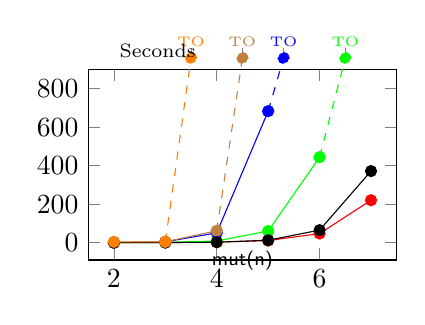
\begin{tikzpicture}
	\begin{axis}[name=Mutex,height=4cm,width=5.5cm,
		xlabel=\scriptsize{\textsf{mut(n)}},
		ylabel=\scriptsize{Seconds},
		x label style={at={(axis description cs:0.5,0.1)},anchor=north},
    	    y label style={at={(axis description cs:0.07,1.1)},anchor=west,rotate=-90},
    	%xmax=9,
		ymax=900,
		clip=false,
         %legend pos=north east
		]
    %exp2
	\addplot[color=red,mark=*] coordinates {
		(2, 0.461)
		(3, 0.877)
		(4, 2.945)
		(5, 11.05)
		(6, 47.634)
		(7, 220.863)
	};
	%exp4
	\addplot[color=green,mark=*] coordinates {
		(2, 0.483)
		(3, 1.602)
		(4, 9.032)
		(5, 60.845)
		(6, 444.691)
		%(6.5, 960) %time out
	};
	\addplot[color=green,mark=*,dashed] coordinates {		
		(6, 444.691)
		(6.5, 960) %time out
	}node[pin={[pin distance=-0.1cm]90:{\tiny{TO}}}]{};
	
	%exp8
	\addplot[color=blue,mark=*] coordinates {
		(2,0.983)
		(3,4.693)
		(4,51.233)
		(5,683.642)
		%(5.3,960) % time out
		%(7,1000)
		%(8,80.27)
		% (9,3600)
	};
	\addplot[color=blue,mark=*,dashed] coordinates {		
		(5,683.642)
		(5.3,960) % time out
		%(7,1000)
		%(8,80.27)
		% (9,3600)
	}node[pin={[pin distance=-0.1cm]90:{\tiny{TO}}}]{};
	
	%lineal10
	\addplot[color=brown,mark=*] coordinates {
		(2,0.608)
		(3,5.016)
		(4,62.034)
		%(4.5,960) % time out
		%(6,2.6)
		%(7,13.12)
		%(8,80.27)
		% (9,3600)
	};
	\addplot[color=brown,mark=*,dashed] coordinates {
		%(2,0.608)
		%(3,5.016)
		(4,62.034)
		(4.5,960) % time out
		%(6,2.6)
		%(7,13.12)
		%(8,80.27)
		% (9,3600)
	}node[pin={[pin distance=-0.1cm]90:{\tiny{TO}}}]{};
	%nocex
	\addplot[color=black,mark=*] coordinates {
		(2,0.348)
		(3,0.75)
		(4,2.679)
		(5,12.971)
		(6,65.403)
		(7,372.247)
		%(8,80.27)
		% (9,3600)
	};
	%psketch
	\addplot[color=orange,mark=*] coordinates {
		(2,4.62)
		(3,4.664)
		%(3.5,960)
		%(5,12.971)
		%(6,65.403)
		%(7,372.247)
		%(8,80.27)
		% (9,3600)
	};
	\addplot[color=orange,mark=*,dashed] coordinates {
		%(2,4.62)
		(3,4.664)
		(3.5,960)
		%(5,12.971)
		%(6,65.403)
		%(7,372.247)
		%(8,80.27)
		% (9,3600)
	}node[pin={[pin distance=-0.1cm]90:{\tiny{TO}}}]{};
	
	 %\addplot[color=black,mark=*] coordinates {
	% 	(9,3600)
	% } node[pin=180:{TO}]{};
	% \addplot[color=blue,dashed] coordinates {
	% 	(8,300)
	% 	(9,200)
	 %} node[pin=300:{TO}]{};
	%\addplot[color=green,mark=*,dashed] coordinates {
	%	(7,310)
		%(9, 107)
	%	} node[pin=180:{TO}]{};
	%\legend{exp2, exp4,exp8,lineal10,nocex}
	%\node[above right] at (rel axis cs:1, 1.1) {Time out:};
	%\node[above right] at (rel axis cs:0, 1) {\;\;\scriptsize{T.O:}};
	\end{axis}
\end{tikzpicture}
\label{fig:comparison}
% PHILOSOPHERS
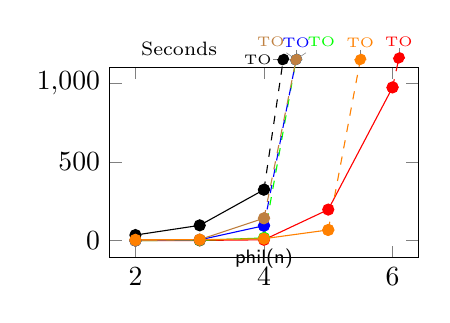
\begin{tikzpicture}
	\begin{axis}[name=Philosophers,height=4cm,width=5.5cm,
		xlabel=\scriptsize{\textsf{phil(n)}},
		ylabel=\scriptsize{Seconds},
		ymax=1100,
		clip=false,
		x label style={at={(axis description cs:0.5,0.1)},anchor=north},
    	y label style={at={(axis description cs:0.07,1.1)},anchor=west,rotate=-90},
		legend pos=north west]
    %exp2
	\addplot[color=red,mark=*] coordinates {
		(2,1.117)
		(3, 1.808)
		(4, 5.987)
		(5,197.652)
		(6,973.321)
		%(6.1,1160)
	};
	\addplot[color=red,mark=*,dashed] coordinates {
		(6,973.321)
		(6.1,1160)
	}node[pin={[pin distance=-0.1cm]90:{\tiny{TO}}}]{};
	%exp4
	\addplot[color=green,mark=*] coordinates {
		(2,1.253)
		(3, 2.765)
		(4, 17.661)
		%(4.5,1150)
		%(6,973.321)
		%(7,1000)
	};
	\addplot[color=green,mark=*,dashed] coordinates {
		(4, 17.661)
		(4.5,1150)
		%(6,973.321)
		%(7,1000)
	}node[pin={[pin distance=-0.1cm]60:{\tiny{TO}}}]{};
	
	%exp8
	\addplot[color=blue,mark=*] coordinates {
		(2,1.37)
		(3,5.552)
		(4,95.327)
		%(4.5,1150)
	     % (8,3600)
	};
	\addplot[color=blue,mark=*,dashed] coordinates {
		(4,95.327)
		(4.5,1150)
	     % (8,3600)
	}node[pin={[pin distance=-0.1cm]90:{\tiny{TO}}}]{};
	%lineal10
	\addplot[color=brown,mark=*] coordinates {
		(2,1.37)
		(3,7.264)
		(4,142.584)
		%(4.5,1150)
	     % (8,3600)
	};
	\addplot[color=brown,mark=*,dashed] coordinates {
		(4,142.584)
		(4.5,1150)
	     % (8,3600)
	}node[pin={[pin distance=-0.1cm]120:{\tiny{TO}}}]{};
	%nocex
	\addplot[color=black,mark=*] coordinates {
		(2,35.998)
		(3,97.636)
		(4,324)
		%(4.3,1150)
	     % (8,3600)
	};
	\addplot[color=black,mark=*,dashed] coordinates {
		(4,324)
		(4.3,1150)
	     % (8,3600)
	}node[pin={[pin distance=-0.1cm]180:{\tiny{TO}}}]{};
	%pskecth
	\addplot[color=orange,mark=*] coordinates {
		(2,5.916)
		(3,6.273)
		(4,12.845)%TO
		 (5,  68.5)
	     %(5.5,1150)
	};
	\addplot[color=orange,mark=*, dashed] coordinates {
		 (5,  68.5)
	     (5.5,1150)
	}node[pin={[pin distance=-0.1cm]90:{\tiny{TO}}}]{};
%\legend{exp2, PSketch}
     %\node[above right] at (rel axis cs:0, 1) {\;\;\scriptsize{T.O.:}};
	\end{axis}
\end{tikzpicture}
% BARRIER
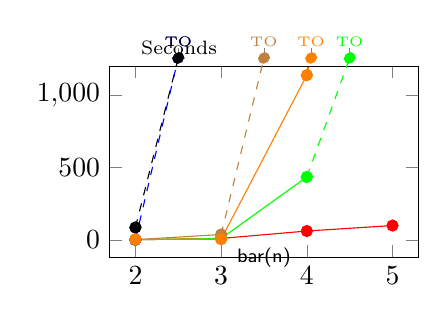
\begin{tikzpicture}
	\begin{axis}[name=SenseBarrier,height=4cm,width=5.5cm,
		xlabel=\scriptsize{\textsf{bar(n)}},
		ylabel=\scriptsize{Seconds},
		ymax=1200,
		clip=false,
		x label style={at={(axis description cs:0.5,0.1)},anchor=north},
    	y label style={at={(axis description cs:0.07,1.1)},anchor=west,rotate=-90},
		legend pos=north west]
    %exp2
	\addplot[color=red,mark=*] coordinates {
	    
		(2,1.535)
		(3, 10.761)
		(4, 62.111)
		(5,100)
		
	};
	%exp4
	\addplot[color=green,mark=*] coordinates {
	
		(2,1.672)
		(3, 10.569)
		(4, 436.365)
		%(4.5,1260) % TO
		%(6,973.321)
		%(7,1000)
	};
	\addplot[color=green,mark=*,dashed] coordinates {
		(4, 436.365)
		(4.5,1260) % TO
		%(6,973.321)
		%(7,1000)
	}node[pin={[pin distance=-0.1cm]90:{\tiny{TO}}}]{};
	
	%exp8
	\addplot[color=blue,mark=*] coordinates {
		(2,2.304)
	%	(2.5,1260)%TO
		%(4,95.327)
		%(5,1150)
	     % (8,3600)
	};
	\addplot[color=blue,mark=*,dashed] coordinates {
		(2,2.304)
		(2.5,1260)%TO
		%(4,95.327)
		%(5,1150)
	     % (8,3600)
	}node[pin={[pin distance=-0.1cm]90:{\tiny{TO}}}]{};
	%lineal10
	\addplot[color=brown,mark=*] coordinates {
	
		(2,2.362)
		(3,37.755)
		%(3.5,1260) % TO
		%(5,1150)
	     % (8,3600)
	};
	\addplot[color=brown,mark=*,dashed] coordinates {
	
		%(2,2.362)
		(3,37.755)
		(3.5,1260) % TO
		%(5,1150)
	     % (8,3600)
	}node[pin={[pin distance=-0.1cm]90:{\tiny{TO}}}]{};
	%nocex
	\addplot[color=black,mark=*] coordinates {
	   
		(2,86.916)
		%(2.5,1260)% TO
		%(4,324)
		%(4.3,1150)
	     % (8,3600)
	};
	\addplot[color=black,mark=*,dashed] coordinates {
	   
		(2,86.916)
		(2.5,1260)% TO
		%(4,324)
		%(4.3,1150)
	     % (8,3600)
	}node[pin={[pin distance=-0.1cm]90:{\tiny{TO}}}]{};
	%PSkecth
	\addplot[color=orange,mark=*] coordinates {
		(2,4.233)
		(3, 5.31)% TO
		(4,1140.9)
		%(4.05,1260)
	     % (8,3600)
	};
	\addplot[color=orange,mark=*,dashed] coordinates {
		(4,1140.9)
		(4.05,1260)
	     % (8,3600)
	}node[pin={[pin distance=-0.1cm]90:{\tiny{TO}}}]{};
%\legend{exp2, PSketch}
    %\node[above right] at (rel axis cs:0, 1) {\;\;\scriptsize{T.O.:}};
	\end{axis}
\end{tikzpicture}

% READERS & WRITERS
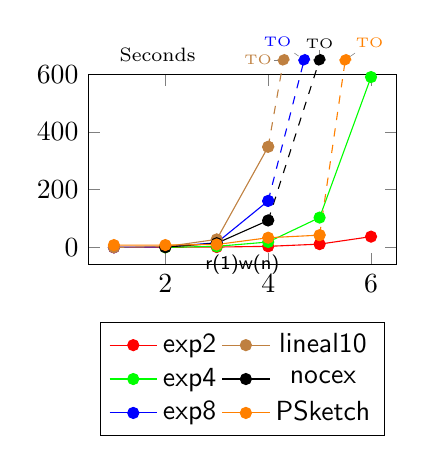
\begin{tikzpicture}
	\begin{axis}[name=Readers and Writers,height=4cm,width=5.5cm,
		xlabel=\scriptsize{\textsf{r(1)w(n)}},
		ylabel=\scriptsize{Seconds},
		x label style={at={(axis description cs:0.5,0.1)},anchor=north},
    	y label style={at={(axis description cs:0.07,1.1)},anchor=west,rotate=-90},
    	ymax=600,
		clip=false,
		legend style={at={(0.5,-0.3)},anchor=north,legend  columns =3, transpose legend}]
    % exp2
     \addlegendimage{red, line legend, mark=*} % or mark=none?
    \addlegendentry{\textsf{exp2}}
    \addlegendimage{green, line legend, , mark=*} % or mark=none?
    \addlegendentry{\textsf{exp4}}
    \addlegendimage{blue, line legend, , mark=*} % or mark=none?
    \addlegendentry{\textsf{exp8}}
    \addlegendimage{brown, line legend, , mark=*} % or mark=none?
    \addlegendentry{\textsf{lineal10}}
    \addlegendimage{black,,line legend,  mark=*} % or mark=none?
    \addlegendentry{\textsf{nocex}}
    \addlegendimage{orange,,line legend,  mark=*} % or mark=none?
    \addlegendentry{\textsf{PSketch}}
	\addplot[color=red,mark=*] coordinates {
		(1,0.492)
		(2,0.813)
		(3,1.603)
		(4,4.069)
		(5,11.705)
		(6,37.703)
	};
	% exp4
	\addplot[color=green,mark=*] coordinates {
		%(1,0.439)
		(2,0.442)
		(3,4.055)
		(4,19.064)
		(5,103.635)
		(6,590.277)
	};
	% exp8
	\addplot[color=blue,mark=*] coordinates {
		(1,0.625)
		(2,2.247)
		(3,16.51)
		(4,161.499)
		%(5,600) %TO
	};
	\addplot[color=blue,mark=*,dashed] coordinates {
		(4,161.499)
		(4.7,650) %TO
	}node[pin={[pin distance=-0.1cm]130:{\tiny{TO}}}]{};
	%lineal10
	\addplot[color=brown,mark=*] coordinates {
		(1,0.654)
		(2,2.892)
		(3,28.208)
		(4,348.931)
		%(4.3,660) %TO
	};
	\addplot[color=brown,mark=*,dashed] coordinates {
		(4,348.931)
		(4.3,650) %TO
	}node[pin={[pin distance=-0.1cm]180:{\tiny{TO}}}]{};
	\addplot[color=black,mark=*] coordinates {
		%(1,0.511)
		(2,1.344)
		(3,14.807)
		(4,93.844)
		%(5,600) %TO
	};
	\addplot[color=black,mark=*,dashed] coordinates {
		%(1,0.511)
		(4,93.844)
		(5,650) %TO
	}node[pin={[pin distance=-0.1cm]90:{\tiny{TO}}}]{};
	
	%PSketch
	\addplot[color=orange,mark=*] coordinates {
		(1,8.465)
		(2,8.483)
		(3,10.463)
		(4,33.898)
		(5,42.824)
		%(6,600)%TO
	};
	\addplot[color=orange,mark=*,dashed] coordinates {
		(5,42.824)
		(5.5,650)%TO
	}node[pin={[pin distance=-0.1cm]70:{\tiny{TO}}}]{};
   %\legend{exp2,exp4,exp8,lineal10,nocex,psketch}
    %\node[above right] at (rel axis cs:0, 1) {\;\;\scriptsize{T.O.:}};
	\end{axis}
\end{tikzpicture}
\vspace{0.4cm}
\captionof{figure}{Comparison between \\ \textsf{exp2}, \textsf{exp4}, \textsf{exp8},  \textsf{lineal10},  \textsf{nocex}, \\ and {\PSketch}.}
\label{fig:examples-plot}
\end{minipage}
\end{tabular}
\vspace{-0.5cm}
\end{table}
}
%{\scriptsize
%\begin{table}[!ht]
%\begin{tabular}{l l}
%\begin{minipage}{0.67\linewidth}
%    \centering
%    \begin{tabular}{|l|l|l|l|l|l|l|l|}
%    \hline
%        Ex. & Sc. & L.Time & G.Time & It. & R.St. & T.St. & Res. \\ \hline
%        Arb2 & 12 & 0.814 &  1.322 & 7 & $2^{2.32}$  & $2^{12}$ & F \\ \hline
%        Arb3 & 12 & 0.728 & 2.11 & 16 & $2^4$ & $2^18$ & F \\ \hline
%        Arb4 & 12 & 0.854 & 4.303 & 16 & $2^{5.24}$ & $2^{24}$ & F \\ \hline
%        Arb5 & 12 & 0.976 & 12.54 & 16 & $2^{6.35}$ & $2^{30}$ & F \\ \hline
%        Arb6 & 12 & 1.134 & 52.344 & 16 & $2^{7.40}$ & $2^{36}$ & F \\ \hline
%        FArb2 & 12 & 0.552 & 1.164 & 8 & $2^{2.58}$ & $2^{12}$ & F \\ \hline
%        FArb3 & 12 & 0.75 & 2.97 & 20 & $2^{3.45}$ & $2^{18}$ & F \\ \hline
%        FArb4 & 12 & 0.935 & 15.602 & 56 & $2^{4.39}$ & $2^{24}$ & F \\ \hline
%        FArb5 & 12 & 1.232 & 85.933 & 164 & $2^{5.35}$ & $2^{30}$ & F \\ \hline
%        FArb6 & 12 & 2.034 & 1004.49 & 857 & - & - & NF\\ \hline
%        FArb2 & 12 & 0.662 & 1.166 & 8 & $2^{2.80}$ & $2^{12}$ & F\\ \hline
%        PArb3 & 12 & 0.714 & 2.277 & 20 & $2^{3.45}$ & $2^{18}$ & F \\ \hline
%        PArb4 & 12 & 0.886 & 8.593 & 56 & $2^{4.39}$ & $2^{24}$ & F\\ \hline
%        PArb5 & 12 & 1.092 & 54.25 & 164 & $2^{5.35}$ & $2^{30}$ & F \\ \hline
%        PArb6 & 12 &1.324 & 700.731 & 488 & $2^{6.33}$ & $2^{36}$ & F \\ \hline
%    \end{tabular}
%\caption{Results for the Arbiter examples.}\label{tab:results-arbiter}
%\end{minipage}
%\begin{minipage}{0.50\linewidth}
%\centering
%\begin{tikzpicture}
%	\begin{axis}[name=Arbiter,height=4cm,width=5.5cm,
%		xlabel=\scriptsize{Arbiter(n)},
%		ylabel=\scriptsize{Seconds},
%		x label style={at={(axis description cs:0.5,0.1)},anchor=north},
%    	y label style={at={(axis description cs:0.07,1.1)},anchor=west,rotate=-90},
%    	ymax=75,
%		clip=false,
%		legend pos=north west]
%    % exp2
%	\addplot[color=red,mark=*] coordinates {
%		(2,0.768)
%		(3,1.563)
%		(4,2.175)
%		(5,3.768)
%		(6,9.172)
%		%(6,37.703)
%	};
%	% exp4
%	\addplot[color=green,mark=*] coordinates {
%		(2,0.78)
%		(3,1.687)
%		(4,3.085)
%		(5,6.985)
%		(6,19.659)
%	};
%	% exp8
%	\addplot[color=blue,mark=*] coordinates {
%		(2,0.67)
%		(3,2.132)
%		(4,4)
%		(5,10.624)
%		(6, 35.653) 
%	};
%	%lineal10
%	\addplot[color=brown,mark=*] coordinates {
%		(2,0.972)
%		(3,3.359)
%		(4,7.829)
%		(5,16.491)
%		(6,54.652)
%	};
%	%Party
%	\addplot[color=pink,mark=*] coordinates {
%		(2,0.63)
%		(3,1.18)
%		(4,2.82)
%		(5,6.12)
%		(6,12.43)
%	};
%	%nocex
%	%\addplot[color=black,mark=x] coordinates {
%	%	(1,0.511)
%	%	(2,1.344)
%	%	(3,14.807)
%	%	(4,93.844)
%	%	(5,600) %TO
%	%};
%	
%%\legend{exp2,exp4,exp8,lineal10,nocex}
%    \node[above right] at (rel axis cs:0, 1) {\;\;\scriptsize{Time out:}};
%	\end{axis}
%\end{tikzpicture}
%%Full Arbiter
%\begin{tikzpicture}
%	\begin{axis}[name=FullArbiter,height=4cm,width=5.5cm,
%		xlabel=\scriptsize{FullArbiter(n)},
%		ylabel=\scriptsize{Seconds},
%		x label style={at={(axis description cs:0.5,0.1)},anchor=north},
%    	y label style={at={(axis description cs:0.07,1.1)},anchor=west,rotate=-90},
%    	ymax=1200,
%		clip=false,
%		legend pos=north west]
%    % exp2
%	\addplot[color=red,mark=*] coordinates {
%		(2,1.164)
%		(3,2.97)
%		(4,15.609)
%		(5,85.933)
%		(6,1004.49)
%		%(6,37.703)
%	};
%	% exp4
%	\addplot[color=green,mark=*] coordinates {
%		(2,0.8)
%		(3,1.466)
%		(4,3.457)
%		(5,10.8)
%		(6,66.433)
%	};
%	% exp8
%	\addplot[color=blue,mark=*] coordinates {
%		(2,0.83)
%		(3,1.507)
%		(4,3.562)
%		(5,12.345)
%		(6, 69.144) %TO
%	};
%	%lineal10
%	\addplot[color=brown,mark=*] coordinates {
%		(2,2.024)
%		(3,19.822)
%		(4,298.955)
%		(5,1200)%TO
%	};
%	\addplot[color=pink,mark=*] coordinates {
%		(2,0.68)
%		(3,1.43)
%		(4,4.078)
%		(5,8.85)
%		(6,32.73)
%	};
%	%nocex
%	%\addplot[color=black,mark=x] coordinates {
%	%	(1,0.511)
%	%	(2,1.344)
%	%	(3,14.807)
%	%	(4,93.844)
%	%	(5,600) %TO
%	%};
%%\legend{exp2,exp4,exp8,lineal10,nocex}
%    \node[above right] at (rel axis cs:0, 1) {\;\;\scriptsize{Time out:}};
%	\end{axis}
%\end{tikzpicture}
%%PNUELIARBITER
%\begin{tikzpicture}
%	\begin{axis}[name=PnueliArbiter,height=4cm,width=5.5cm,
%		xlabel=\scriptsize{PnueliArbiter(n)},
%		ylabel=\scriptsize{Seconds},
%		x label style={at={(axis description cs:0.5,0.1)},anchor=north},
%    	y label style={at={(axis description cs:0.07,1.1)},anchor=west,rotate=-90},
%    	ymax=1400,
%		clip=false,
%		legend style={at={(0.2,-0.5)},anchor=north}]
%    % exp2
%	\addplot[color=red,mark=*] coordinates {
%		(2,1.168)
%		(3,2.277)
%		(4,8.593)
%		(5,54.25)
%		(6,1362.85) % TO
%		%(6,37.703)
%	};
%	% exp4
%	\addplot[color=green,mark=*] coordinates {
%		(2,0.676)
%		(3,1.146)
%		(4,2.355)
%		(5,11.6)
%		(6,66.433) 
%	};
%	% exp8
%	\addplot[color=blue,mark=*] coordinates {
%		(2,0.707)
%		(3,1.242)
%		(4,2.433)
%		(5,12.173)
%		(6, 65.155) %TO
%	};
%	%lineal10
%	\addplot[color=brown,mark=*] coordinates {
%		(2,0.69)
%		(3,1.162)
%		(4,2.408)
%		(5,11.836)
%		(6,59.299)
%	};
%	%nocex
%	%\addplot[color=black,mark=x] coordinates {
%	%	(1,0.511)
%	%	(2,1.344)
%	%	(3,14.807)
%	%	(4,93.844)
%	%	(5,600) %TO
%	%};
%	%party
%	\addplot[color=pink,mark=*] coordinates {
%		(2,0.69)
%		(3,1.162)
%		(4,2.408)
%		(5,11.836)
%		(6,1400)
%	};
%\legend{exp2,exp4,exp8,lineal10,nocex}
%    \node[above right] at (rel axis cs:0, 1) {\;\;\scriptsize{Time out:}};
%	\end{axis}
%\end{tikzpicture}
%\end{minipage}
%\end{tabular}
%\end{table}
%}

%\begin{figure}[hbt!]
%\begin{tabular}{l l}
%\begin{minipage}{0.48\linewidth}
%\centering
%%MUTEX
%\begin{tikzpicture}
%	\begin{axis}[name=Mutex,height=4cm,width=5.5cm,
%		xlabel=\scriptsize{Mutex(n)},
%		ylabel=\scriptsize{Seconds},
%		x label style={at={(axis description cs:0.5,0.1)},anchor=north},
%    	    y label style={at={(axis description cs:0.07,1.1)},anchor=west,rotate=-90},
%    	%xmax=9,
%		ymax=900,
%		clip=false,
%         %legend pos=north east
%		]
%    %exp2
%	\addplot[color=red,mark=*] coordinates {
%		(2, 0.461)
%		(3, 0.877)
%		(4, 2.945)
%		(5, 11.05)
%		(6, 47.634)
%		(7, 220.863)
%	};
%	%exp4
%	\addplot[color=green,mark=*] coordinates {
%		(2, 0.483)
%		(3, 1.602)
%		(4, 9.032)
%		(5, 60.845)
%		(6, 444.691)
%		(7, 900) %time out
%	};
%	%exp8
%	\addplot[color=blue,mark=*] coordinates {
%		(2,0.983)
%		(3,4.693)
%		(4,51.233)
%		(5,683.642)
%		(5.3,900) % time out
%		%(7,1000)
%		%(8,80.27)
%		% (9,3600)
%	};
%	%lineal10
%	\addplot[color=brown,mark=*] coordinates {
%		(2,0.608)
%		(3,5.016)
%		(4,62.034)
%		(5,900) % time out
%		%(6,2.6)
%		%(7,13.12)
%		%(8,80.27)
%		% (9,3600)
%	};
%	%nocex
%	\addplot[color=black,mark=*] coordinates {
%		(2,0.348)
%		(3,0.75)
%		(4,2.679)
%		(5,12.971)
%		(6,65.403)
%		(7,372.247)
%		%(8,80.27)
%		% (9,3600)
%	};
%	 %\addplot[color=black,mark=*] coordinates {
%	% 	(9,3600)
%	% } node[pin=180:{TO}]{};
%	% \addplot[color=blue,dashed] coordinates {
%	% 	(8,300)
%	% 	(9,200)
%	 %} node[pin=300:{TO}]{};
%	%\addplot[color=green,mark=*,dashed] coordinates {
%	%	(7,310)
%		%(9, 107)
%	%	} node[pin=180:{TO}]{};
%	%\legend{exp2, exp4,exp8,lineal10,nocex}
%	%\node[above right] at (rel axis cs:1, 1.1) {Time out:};
%	\node[above right] at (rel axis cs:0, 1) {\;\;\scriptsize{Time out:}};
%	\end{axis}
%\end{tikzpicture}
%\label{fig:comparison}
%% PHILOSOPHERS
%\begin{tikzpicture}
%	\begin{axis}[name=Philosophers,height=4cm,width=5.5cm,
%		xlabel=\scriptsize{Phils(n)},
%		ylabel=\scriptsize{Seconds},
%		ymax=1100,
%		clip=false,
%		x label style={at={(axis description cs:0.5,0.1)},anchor=north},
%    	y label style={at={(axis description cs:0.07,1.1)},anchor=west,rotate=-90},
%		legend pos=north west]
%    %exp2
%	\addplot[color=red,mark=*] coordinates {
%		(2,1.117)
%		(3, 1.808)
%		(4, 5.987)
%		(5,197.652)
%		(6,973.321)
%		(6.1,1100)
%	};
%	%exp4
%	\addplot[color=green,mark=*] coordinates {
%		(2,1.253)
%		(3, 2.765)
%		(4, 17.661)
%		(5,1100)
%		%(6,973.321)
%		%(7,1000)
%	};
%	%exp8
%	\addplot[color=blue,mark=*] coordinates {
%		(2,1.37)
%		(3,5.552)
%		(4,95.327)
%		(5,1100)
%	     % (8,3600)
%	};
%	%lineal10
%	\addplot[color=brown,mark=*] coordinates {
%		(2,1.37)
%		(3,7.264)
%		(4,142.584)
%		(5,1100)
%	     % (8,3600)
%	};
%	%nocex
%	\addplot[color=black,mark=*] coordinates {
%		(2,35.998)
%		(3,97.636)
%		(4,324)
%		(4.3,1100)
%	     % (8,3600)
%	};
%%\legend{exp2, PSketch}
%     \node[above right] at (rel axis cs:0, 1) {\;\;\scriptsize{Time out:}};
%	\end{axis}
%\end{tikzpicture}
%% BARRIER
%\begin{tikzpicture}
%	\begin{axis}[name=SenseBarrier,height=4cm,width=5.5cm,
%		xlabel=\scriptsize{SenseBarrier(n)},
%		ylabel=\scriptsize{Seconds},
%		ymax=500,
%		clip=false,
%		x label style={at={(axis description cs:0.5,0.1)},anchor=north},
%    	y label style={at={(axis description cs:0.07,1.1)},anchor=west,rotate=-90},
%		legend pos=north west]
%    %exp2
%	\addplot[color=red,mark=*] coordinates {
%	    
%		(2,1.535)
%		(3, 10.761)
%		(4, 62.111)
%		(5,100)
%		
%	};
%	%exp4
%	\addplot[color=green,mark=*] coordinates {
%	
%		(2,1.672)
%		(3, 10.569)
%		(4, 436.365)
%		(4.1,500) % TO
%		%(6,973.321)
%		%(7,1000)
%	};
%	%exp8
%	\addplot[color=blue,mark=*] coordinates {
%	
%		(2,2.304)
%		(3,500)%TO
%		%(4,95.327)
%		%(5,1150)
%	     % (8,3600)
%	};
%	%lineal10
%	\addplot[color=brown,mark=*] coordinates {
%	
%		(2,2.362)
%		(3,37.755)
%		(4,500) % TO
%		%(5,1150)
%	     % (8,3600)
%	};
%	%nocex
%	\addplot[color=black,mark=*] coordinates {
%	   
%		(2,86.916)
%		(2.5,500)% TO
%		%(4,324)
%		%(4.3,1150)
%	     % (8,3600)
%	};
%%\legend{exp2, PSketch}
%    \node[above right] at (rel axis cs:0, 1) {\;\;\scriptsize{Time out:}};
%	\end{axis}
%\end{tikzpicture}
%
%% READERS & WRITERS
%\begin{tikzpicture}
%	\begin{axis}[name=Readers and Writers,height=4cm,width=5.5cm,
%		xlabel=\scriptsize{RW(1,n)},
%		ylabel=\scriptsize{Seconds},
%		x label style={at={(axis description cs:0.5,0.1)},anchor=north},
%    	y label style={at={(axis description cs:0.07,1.1)},anchor=west,rotate=-90},
%    	ymax=600,
%		clip=false,
%		legend pos=north west]
%    % exp2
%	\addplot[color=red,mark=*] coordinates {
%		(1,0.492)
%		(2,0.813)
%		(3,1.603)
%		(4,4.069)
%		(5,11.705)
%		(6,37.703)
%	};
%	% exp4
%	\addplot[color=green,mark=*] coordinates {
%		(1,0.439)
%		(2,0.442)
%		(3,4.055)
%		(4,19.064)
%		(5,103.635)
%		(6,590.277)
%	};
%	% exp8
%	\addplot[color=blue,mark=*] coordinates {
%		(1,0.625)
%		(2,2.247)
%		(3,16.51)
%		(4,161.499)
%		(5,600) %TO
%	};
%	%lineal10
%	\addplot[color=brown,mark=*] coordinates {
%		(1,0.654)
%		(2,2.892)
%		(3,28.208)
%		(4,348.931)
%		(4.3,600) %TO
%	};
%	\addplot[color=black,mark=*] coordinates {
%		(1,0.511)
%		(2,1.344)
%		(3,14.807)
%		(4,93.844)
%		(5,600) %TO
%	};
%
%%\legend{exp2,exp4,exp8,lineal10,nocex}
%    \node[above right] at (rel axis cs:0, 1) {\;\;\scriptsize{Time out:}};
%	\end{axis}
%\end{tikzpicture}
%\end{minipage}
%%\captionof{figure}{Comparison for exp2, exp4, exp8, lineal10, and nocex.}
%&
%%%% ARBITER EXAMPLES
%%Arbiter
%\begin{minipage}{0.48\linewidth}
%\centering
%\begin{tikzpicture}
%	\begin{axis}[name=Arbiter,height=4cm,width=5.5cm,
%		xlabel=\scriptsize{Arbiter(n)},
%		ylabel=\scriptsize{Seconds},
%		x label style={at={(axis description cs:0.5,0.1)},anchor=north},
%    	y label style={at={(axis description cs:0.07,1.1)},anchor=west,rotate=-90},
%    	ymax=75,
%		clip=false,
%		legend pos=north west]
%    % exp2
%	\addplot[color=red,mark=*] coordinates {
%		(2,0.768)
%		(3,1.563)
%		(4,2.175)
%		(5,3.768)
%		(6,9.172)
%		%(6,37.703)
%	};
%	% exp4
%	\addplot[color=green,mark=*] coordinates {
%		(2,0.78)
%		(3,1.687)
%		(4,3.085)
%		(5,6.985)
%		(6,19.659)
%	};
%	% exp8
%	\addplot[color=blue,mark=*] coordinates {
%		(2,0.67)
%		(3,2.132)
%		(4,4)
%		(5,10.624)
%		(6, 35.653) 
%	};
%	%lineal10
%	\addplot[color=brown,mark=*] coordinates {
%		(2,0.972)
%		(3,3.359)
%		(4,7.829)
%		(5,16.491)
%		(6,54.652)
%	};
%	%Party
%	\addplot[color=pink,mark=*] coordinates {
%		(2,0.63)
%		(3,1.18)
%		(4,2.82)
%		(5,6.12)
%		(6,12.43)
%	};
%	%nocex
%	%\addplot[color=black,mark=x] coordinates {
%	%	(1,0.511)
%	%	(2,1.344)
%	%	(3,14.807)
%	%	(4,93.844)
%	%	(5,600) %TO
%	%};
%	
%%\legend{exp2,exp4,exp8,lineal10,nocex}
%    \node[above right] at (rel axis cs:0, 1) {\;\;\scriptsize{Time out:}};
%	\end{axis}
%\end{tikzpicture}
%%Full Arbiter
%\begin{tikzpicture}
%	\begin{axis}[name=FullArbiter,height=4cm,width=5.5cm,
%		xlabel=\scriptsize{FullArbiter(n)},
%		ylabel=\scriptsize{Seconds},
%		x label style={at={(axis description cs:0.5,0.1)},anchor=north},
%    	y label style={at={(axis description cs:0.07,1.1)},anchor=west,rotate=-90},
%    	ymax=1200,
%		clip=false,
%		legend pos=north west]
%    % exp2
%	\addplot[color=red,mark=*] coordinates {
%		(2,1.164)
%		(3,2.97)
%		(4,15.609)
%		(5,85.933)
%		(6,1004.49)
%		%(6,37.703)
%	};
%	% exp4
%	\addplot[color=green,mark=*] coordinates {
%		(2,0.8)
%		(3,1.466)
%		(4,3.457)
%		(5,10.8)
%		(6,66.433)
%	};
%	% exp8
%	\addplot[color=blue,mark=*] coordinates {
%		(2,0.83)
%		(3,1.507)
%		(4,3.562)
%		(5,12.345)
%		(6, 69.144) %TO
%	};
%	%lineal10
%	\addplot[color=brown,mark=*] coordinates {
%		(2,2.024)
%		(3,19.822)
%		(4,298.955)
%		(5,1200)%TO
%	};
%	\addplot[color=pink,mark=*] coordinates {
%		(2,0.68)
%		(3,1.43)
%		(4,4.078)
%		(5,8.85)
%		(6,32.73)
%	};
%	%nocex
%	%\addplot[color=black,mark=x] coordinates {
%	%	(1,0.511)
%	%	(2,1.344)
%	%	(3,14.807)
%	%	(4,93.844)
%	%	(5,600) %TO
%	%};
%%\legend{exp2,exp4,exp8,lineal10,nocex}
%    \node[above right] at (rel axis cs:0, 1) {\;\;\scriptsize{Time out:}};
%	\end{axis}
%\end{tikzpicture}
%%PNUELIARBITER
%\begin{tikzpicture}
%	\begin{axis}[name=PnueliArbiter,height=4cm,width=5.5cm,
%		xlabel=\scriptsize{PnueliArbiter(n)},
%		ylabel=\scriptsize{Seconds},
%		x label style={at={(axis description cs:0.5,0.1)},anchor=north},
%    	y label style={at={(axis description cs:0.07,1.1)},anchor=west,rotate=-90},
%    	ymax=1400,
%		clip=false,
%		legend style={at={(0.2,-0.5)},anchor=north}]
%    % exp2
%	\addplot[color=red,mark=*] coordinates {
%		(2,1.168)
%		(3,2.277)
%		(4,8.593)
%		(5,54.25)
%		(6,1362.85) % TO
%		%(6,37.703)
%	};
%	% exp4
%	\addplot[color=green,mark=*] coordinates {
%		(2,0.676)
%		(3,1.146)
%		(4,2.355)
%		(5,11.6)
%		(6,66.433) 
%	};
%	% exp8
%	\addplot[color=blue,mark=*] coordinates {
%		(2,0.707)
%		(3,1.242)
%		(4,2.433)
%		(5,12.173)
%		(6, 65.155) %TO
%	};
%	%lineal10
%	\addplot[color=brown,mark=*] coordinates {
%		(2,0.69)
%		(3,1.162)
%		(4,2.408)
%		(5,11.836)
%		(6,59.299)
%	};
%	%nocex
%	%\addplot[color=black,mark=x] coordinates {
%	%	(1,0.511)
%	%	(2,1.344)
%	%	(3,14.807)
%	%	(4,93.844)
%	%	(5,600) %TO
%	%};
%	%party
%	\addplot[color=pink,mark=*] coordinates {
%		(2,0.69)
%		(3,1.162)
%		(4,2.408)
%		(5,11.836)
%		(6,1400)
%	};
%\legend{exp2,exp4,exp8,lineal10,nocex}
%    \node[above right] at (rel axis cs:0, 1) {\;\;\scriptsize{Time out:}};
%	\end{axis}
%\end{tikzpicture}
%\vspace{1.3cm}
%
%%\captionof{figure}{Comparison with Party Tool.}
%\label{fig:comparison}
%\end{minipage}
%\end{tabular}
%\end{figure}
We evaluate our approach around the following research questions: 
\begin{description}
\item[RQ1] \emph{How effective/efficient is our synthesis approach?}
\item[RQ2] \emph{How good is the counterexample-guided search for speeding up the synthesis method?}
\item[RQ3] \emph{How do the selected bounds affect the synthesis method?}
\item[RQ4] \emph{How does our approach compare with related approaches?}
\end{description}
To answer these questions,  we implemented Alg.~\ref{alg:improved_alg} in a prototype tool, it uses the \textsf{Alloy Analyzer}~\cite{AlloyBook} for obtaining instances of specifications, and {\NuSMV}~\cite{Cimatti+2002} for model checking the candidates.  We evaluate our approach on eight  examples of distributed algorithms: the dining philosophers (\textsf{phil})~\cite{Dijkstra71} (our running example), Mutex (\textsf{mut})~\cite{Fokkink13},  Readers and Writers (\textsf{rw})~\cite{Fokkink13}, the generalized version of Peterson's algorithm (\textsf{pet})~\cite{Fokkink13},   and the combined-tree Barrier protocol (\textsf{bar})~\cite{Fokkink13}.  Furthermore,  we  also encoded the arbiter examples presented in \cite{Party,Piterman+2006}: a simple arbiter (\textsf{arb}), a full arbiter (\textsf{farb}), and the Pnueli arbiter (\textsf{parb}). These case studies assume a distributed token ring architecture,  which we modeled using the Alloy language.  

%\cite{PhilStone}. The tool takes as input a  specification and returns, when possible, an LTS satisfying the specification, described in the \NuSMV  language.
Tables~\ref{tab:results-common} and~\ref{tab:results-arbiter}  summarize the experimental results. The experiments were conducted on an Apple M2 processor with 16GB of memory.   In these examples, we used the sequence of bounds $2,4,8,16,\dots$, named \textsf{exp2} from now on.
For each case study, we report the 
bound over the size of the processes (Sc), the maximum time needed to generate local process instances (L.Time), the total time required for synthesizing the system (T.Time), the number of times that the model checker was invoked (Its) by the synthesizer, and the final result of our synthesis algorithm:  `F' (if an implementation was found),  `N'  (if no implementation was found),  `TO'  if the example timed out, or `U'  (if the specification was found unsatisfiable by the Alloy tool).  We also report the number of reachable states (R.St.), and the total states (T.St.) of the obtained implementations, expressed as power of $2$.  For space reasons, we only include a few configurations found unsatisfiable by the solver; similar numbers can be obtained for the rest of the cases if the specifications are processed with smaller scopes. We also indicate the number of processes considered in each experiment.  For instance,  \textsf{phil(6)} indicates that we considered \textsf{6} concurrent processes (i.e., philosophers) in the dining philosophers example. In the case of Readers and Writers, 
\textsf{r(n)w(m)} means that \textsf{n} readers and \textsf{m} writers were considered.  We  have  set out a time out of 30 minutes.
\begin{wraptable}[19]{r}{.60\textwidth}
\vspace{-0.5cm}
\begin{tabular}{|l|l|l|l|l|l|l|l|}
    \hline
        Ex. & Sc. & L.Time & G.Time & It. & R.St. & T.St. & Res. \\ \hline
        \textsf{arb(2)} & 12 & 0.814 &  1.322 & 7 & $2^{2.32}$  & $2^{12}$ & F \\ \hline
        \textsf{arb(3)} & 12 & 0.728 & 2.11 & 16 & $2^4$ & $2^{18}$ & F \\ \hline
        \textsf{arb(4)} & 12 & 0.854 & 4.303 & 16 & $2^{5.24}$ & $2^{24}$ & F \\ \hline
        \textsf{arb(5)} & 12 & 0.976 & 12.54 & 16 & $2^{6.35}$ & $2^{30}$ & F \\ \hline
        \textsf{arb(6)} & 12 & 1.134 & 52.344 & 16 & $2^{7.40}$ & $2^{36}$ & F \\ \hline
        \textsf{farb(2)} & 12 & 0.552 & 1.164 & 8 & $2^{2.58}$ & $2^{12}$ & F \\ \hline
        \textsf{farb(3)} & 12 & 0.75 & 2.97 & 20 & $2^{3.45}$ & $2^{18}$ & F \\ \hline
        \textsf{farb(4)} & 12 & 0.935 & 15.602 & 56 & $2^{4.39}$ & $2^{24}$ & F \\ \hline
        \textsf{farb(5)} & 12 & 1.232 & 85.933 & 164 & $2^{5.35}$ & $2^{30}$ & F \\ \hline
        \textsf{farb(6)} & 12 & 2.034 & 672.539 & 488 & $2^{6.33}$ & $2^{36}$ & F\\ \hline
        \textsf{parb(2)} & 12 & 0.662 & 1.166 & 8 & $2^{2.80}$ & $2^{12}$ & F\\ \hline
        \textsf{parb(3)} & 12 & 0.714 & 2.277 & 20 & $2^{3.45}$ & $2^{18}$ & F \\ \hline
        \textsf{parb(4)} & 12 & 0.886 & 8.593 & 56 & $2^{4.39}$ & $2^{24}$ & F\\ \hline
        \textsf{parb(5)} & 12 & 1.092 & 54.25 & 164 & $2^{5.35}$ & $2^{30}$ & F \\ \hline
        \textsf{parb(6)} & 12 &1.324 & 700.731 & 488 & $2^{6.33}$ & $2^{36}$ & F \\ \hline
\end{tabular}
\caption{Results for the arbiter examples.}\label{tab:results-arbiter}
\end{wraptable}
%
Table \ref{tab:results-common} shows that the technique scales reasonably well for those case studies in which each process uses only a reduced number of locks and shared variables (e.g., dining philosophers, mutex and reader-writers). For the cases where the number of shared variables accessed by the processes is bigger (e.g., Peterson for $n$ processes), the technique does not scale that well. Intuitively, more shared variables imply more actions performed by the environment, which increases the size of the formula fed to the SAT solver.  We plan to investigate how to equip specifications with assumptions on the environment's behavior, to restrict the possible values of shared variables; this may simplify the SAT problem when searching for local implementations.  It is worth noting, that even though the algorithm is incomplete, we have not 
observed any ``not found'' outputs in our benchmarks. This could be due to  the set timeouts.  We leave an in-depth investigation of this as further work.

 To answer \textbf{RQ3}   we compare the results obtained with several configurations of bounds for the exploration phase, namely: \textsf{exp4} ($4,16,64,\dots$),  \textsf{exp8} ($8,64,512,\dots$),  \textsf{lineal10} ($10,20,30,\dots$), and for \textbf{RQ2} we also considered Alg.~\ref{alg:the_alg},  which does not take into account counterexamples (\textsf{nocex}).  The obtained results are depicted in Figs.\ref{fig:examples-plot} and \ref{fig:arbiter-plots}.  Note that time outs are remarked using dashed lines going out of the $y$-axis.
 In general, \textsf{exp2} behaves better than the other options,  thus it seems better to collect a few counterexamples first, and use them to improve the search.  A possible drawback of this setting is that a wrong choice of the first counterexamples may have as a consequence that no implementation is found,  i.e., one may expect that this configuration  is ``more incomplete''   than the other options. However, we have not observed this in our benchmarks.  Note that \textsf{nocex} timed out in many examples. Indeed, for the arbiter examples, \textsf{nocex} was able only to solve the examples with two processes,  taking for that more than $7000$ iterations.

\begin{wrapfigure}[31]{hr}{.40\textwidth}
\vspace{-1.5cm}
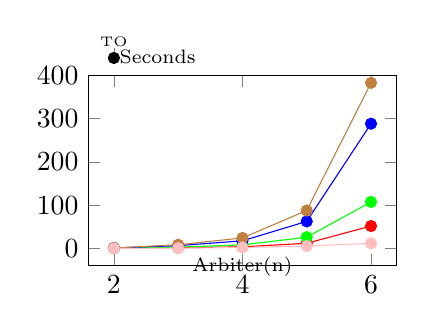
\begin{tikzpicture}
	\begin{axis}[name=Arbiter,height=4cm,width=5.5cm,
		xlabel=\scriptsize{Arbiter(n)},
		ylabel=\scriptsize{Seconds},
		x label style={at={(axis description cs:0.5,0.1)},anchor=north},
    	y label style={at={(axis description cs:0.07,1.1)},anchor=west,rotate=-90},
    	ymax=400,
		clip=false,
		legend pos=north west]
    % exp2
	\addplot[color=red,mark=*] coordinates {
		(2,1.3)
		(3,2.11)
		(4,4.3)
		(5,12.54)
		(6,52.34)
		%(6,37.703)
	};
	% exp4
	\addplot[color=green,mark=*] coordinates {
		(2,1.372)
		(3,3.545)
		(4,8.824)
		(5,26.531)
		(6,107.897)
	};
	% exp8
	\addplot[color=blue,mark=*] coordinates {
		(2,1.72)
		(3,7.022)
		(4,18.176)
		(5,63.028)
		(6, 288.419) 
	};
	%lineal10
	\addplot[color=brown,mark=*] coordinates {
		(2,1.737)
		(3,9.11)
		(4,24.866)
		(5,88.064)
		(6,382.565)
	};
	%Party
	\addplot[color=pink,mark=*] coordinates {
		(2,0.63)
		(3,1.18)
		(4,2.82)
		(5,6.12)
		(6,12.43)
	};
	%nocex
	\addplot[color=black,mark=*] coordinates {
	%	(1,0.511)
		(2,440)
	%	(3,14.807)
	%	(4,93.844)
	%	(5,600) %TO
	}node[pin={[pin distance=-0.1cm]90:{\tiny{TO}}}]{};

%\legend{exp2,exp4,exp8,lineal10,nocex}
    %\node[above right] at (rel axis cs:0, 1) {\;\;\scriptsize{T.O.:}};
	\end{axis}
\end{tikzpicture}
%Full Arbiter
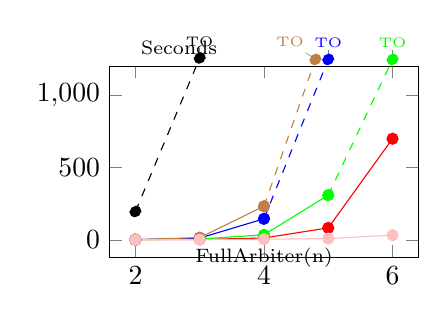
\begin{tikzpicture}
	\begin{axis}[name=FullArbiter,height=4cm,width=5.5cm,
		xlabel=\scriptsize{FullArbiter(n)},
		ylabel=\scriptsize{Seconds},
		x label style={at={(axis description cs:0.5,0.1)},anchor=north},
    	y label style={at={(axis description cs:0.07,1.1)},anchor=west,rotate=-90},
    	ymax=1200,
		clip=false,
		legend pos=north west]
    % exp2
	\addplot[color=red,mark=*] coordinates {
		(2,1.083)
		(3,2.774)
		(4,12.873)
		(5,82.981)
		(6,700.731)
		%(6,37.703)
	};
	% exp4
	\addplot[color=green,mark=*] coordinates {
		(2,1.24)
		(3,5.719)
		(4,34.7)
		(5,309.953)
	};
	\addplot[color=green,mark=*,dashed] coordinates {
		(5,309.953)
		(6,1250)
	}node[pin={[pin distance=-0.1cm]90:{\tiny{TO}}}]{};
	
	% exp8
	\addplot[color=blue,mark=*] coordinates {
		(2,1.55)
		(3,12.382)
		(4,145.86)
	};
	\addplot[color=blue,mark=*,dashed] coordinates {
		(4,145.86)
		(5,1250)
	}node[pin={[pin distance=-0.1cm]90:{\tiny{TO}}}]{};
	
	%lineal10
	\addplot[color=brown,mark=*] coordinates {
		(2,1.677)
		(3,15.45)
		(4,232.942)
		%(5,1250)%TO
	};
	\addplot[color=brown,mark=*,dashed] coordinates {
		(4,232.942)
		(4.8,1250)%TO
	}node[pin={[pin distance=-0.1cm]120:{\tiny{TO}}}]{};
	    
	%Party
	\addplot[color=pink,mark=*] coordinates {
		(2,0.68)
		(3,1.43)
		(4,4.078)
		(5,8.85)
		(6,32.73)
	};
	%nocex
	\addplot[color=black,mark=*,dashed] coordinates {
	%	(1,0.511)
		(2,196.115)
		(3,1260) % TO
	%	(4,93.844)
	%	(5,600) %TO
	}node[pin={[pin distance=-0.1cm]90:{\tiny{TO}}}]{};
	
%\legend{exp2,exp4,exp8,lineal10,nocex}
    %\node[above right] at (rel axis cs:0, 1) {\;\;\scriptsize{T.O.:}};
	\end{axis}
\end{tikzpicture}
%PNUELIARBITER
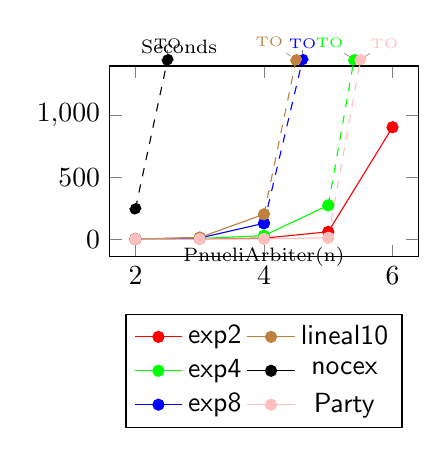
\begin{tikzpicture}
	\begin{axis}[name=PnueliArbiter,height=4cm,width=5.5cm,
		xlabel=\scriptsize{PnueliArbiter(n)},
		ylabel=\scriptsize{Seconds},
		x label style={at={(axis description cs:0.5,0.1)},anchor=north},
    	y label style={at={(axis description cs:0.07,1.1)},anchor=west,rotate=-90},
    	ymax=1400,
		clip=false,
		legend style={at={(0.5,-0.3)},anchor=north,legend  columns =3, transpose legend}]
    % exp2
     \addlegendimage{red, line legend, mark=*} % or mark=none?
    \addlegendentry{\textsf{exp2}}
    \addlegendimage{green, line legend, , mark=*} % or mark=none?
    \addlegendentry{\textsf{exp4}}
    \addlegendimage{blue, line legend, , mark=*} % or mark=none?
    \addlegendentry{\textsf{exp8}}
    \addlegendimage{brown, line legend, , mark=*} % or mark=none?
    \addlegendentry{\textsf{lineal10}}
    \addlegendimage{black,,line legend,  mark=*} % or mark=none?
    \addlegendentry{\textsf{nocex}}
    \addlegendimage{pink,line legend,  mark=*} % or mark=none?
    \addlegendentry{\textsf{Party}}
    % exp2
	\addplot[color=red,mark=*] coordinates {
		(2,1.206)
		(3,2.674)
		(4,8.639)
		(5,59.893)
		(6,905.203) % TO
		%(6,37.703)
	};
	% exp4
	\addplot[color=green,mark=*] coordinates {
		(2,1.406)
		(3,5.461)
		(4,29.063)
		(5,274.013)
	};
	\addplot[color=green,mark=*,dashed] coordinates {
		(5,274.013)
		(5.4,1450) 
	}node[pin={[pin distance=-0.1cm]110:{\tiny{TO}}}]{};
	
	% exp8
	\addplot[color=blue,mark=*] coordinates {
		(2,1.634)
		(3,9.749)
		(4,128.565)
	};
	\addplot[color=blue,mark=*,dashed] coordinates {
		(4,128.565)
		(4.6, 1450) %TO
	}node[pin={[pin distance=-0.1cm]90:{\tiny{TO}}}]{};
	%lineal10
	\addplot[color=brown,mark=*] coordinates {
		(2,1.789)
		(3,13.855)
		(4,201.653)
	};
	\addplot[color=brown,mark=*,dashed] coordinates {	
		(4,201.653)
		(4.5,1450)
	}node[pin={[pin distance=-0.1cm]130:{\tiny{TO}}}]{};
	%nocex
	\addplot[color=black,mark=*,dashed] coordinates {
	%	(1,0.511)
		(2,246.157)
	 	(2.5,1450)
	%	(4,93.844)
	%	(5,600) %TO
	}node[pin={[pin distance=-0.1cm]90:{\tiny{TO}}}]{};
	%party
	\addplot[color=pink,mark=*] coordinates {
		(2,0.69)
		(3,1.162)
		(4,2.408)
		(5,11.836)
		%(5.5,1450)
	};
	\addplot[color=pink,mark=*,dashed] coordinates {
		(5,11.836)
		(5.5,1450)
	}node[pin={[pin distance=-0.1cm]80:{\tiny{TO}}}]{};
    %\legend{exp2,exp4,exp8,lineal10,nocex,Party}
    %\node[above right] at (rel axis cs:0, 1) {\;\;\scriptsize{T.O.:}};
	\end{axis}
\end{tikzpicture}
\caption{Efficiency comparison for arbiter examples}\label{fig:arbiter-plots}
\end{wrapfigure}
To answer \textbf{RQ4} we have included in out analysis the synthesis tool {\PSketch}~\cite{Solar-Lezama+2008}, that implements a Counterexample-driven Guided Inductive Synthesis (CEGIS) algorithm to obtain code from sketched code (i.e., code annotated with ``holes''). To run {\PSketch}, we took the Dining Philosophers specification provided in~\cite{Solar-Lezama+2008}, and manually elaborated the specification for Mutex,  Readers-Writers, and the Barrier example.  The Peterson example cannot be analysed with  {\PSketch} since this tool only supports the analysis of safety properties.  For the arbiter case studies, we have compare against the tool {\Party} \cite{Party} which is a tool specifically tailored for distributed systems that use token ring architectures.

Our comparison focuses only on the time required by each technique for synthesizing the distributed solutions. The plots of Figs.~\ref{fig:examples-plot} and \ref{fig:arbiter-plots} depict the results of this comparison. In all the case studies, we notice that the efficiency of {\PSketch} is drastically affected as the number of processes to synthesize is incremented. For instance, in the dining philosophers with 6 processes, {\Sketch} timed out; in contrast, our tool was able to obtain a solution. Similarly, in the case of 1 reader and 6 writers, {\PSketch} failed in synthesizing a solution, while our approach succeeded. A similar analysis applies to Mutex.

  In the case of the tool {\Party}, for the \textsf{arb} and \textsf{farb} examples {\Party} was able to find solutions faster than \textsf{exp2}; it must be noted that in these cases {\Party} uses a cut-off of $4$,  i.e., it reduces configurations with $n>4$ processes to the case $n=4$.  However,  even though {\Party} has several optimizations for token ring systems, our tool was able to synthesize an implementation of the \textsf{parb(6)} and {\Party} timed out for this case. 
  
It is worth noting that the tool can be used to find different solutions for some examples.  We have experimented with this using the \textsf{phil} example, where, after finding an initial solution, we allow the algorithm to keep looking for further solutions, and it succeeded in finding a second solution.  For space reasons we do not investigate this aspect of the tool further here.

%For instance, for the dining philosophers, the first found solution is one in which each philosopher takes a fork only if her two forks are available (a know solution to prevent deadlock). When we allow the algorithm to keep looking for further solutions, it succeeded in finding a second solution, the ``even/odd'' solution, where $n-1$ philosophers take first their left fork and after their right fork, whereas  philosopher $n$ takes first her right fork and then her left fork.  

\section{Comments and further discussion}
\label{subsec:rst_comment}
\subsection{Accuracy vs discontinuities}
\begin{figure}
\includegraphics[scale=0.50]{images/extra/flow.pdf}
\centering
\vspace{-0.1em}
\caption{Complexity and smoothness trade-off regions of RST algorithm depending on number of blocks and waypoints in each block.}
\vspace{-1.0em}
\label{fig:rst_regions}
\end{figure}
In this section, we present a useful rule of thumb for applying the RST and the RST$_{\text{opt}}$ algorithm according to the number of blocks the user considers and the number of waypoints inside each of these blocks. 
Indeed, Fig.~\ref{fig:rst_regions} and Fig.~\ref{fig:rst_example1} identify regions, suggesting which algorithm to apply according to the number of waypoints and blocks.
So far, most of path planning research has been focused on piecewise polynomial approaches, sticking to the first left strip in Fig.~\ref{fig:rst_regions}. There are, indeed, cases where numerical polynomial complexity is the main concern and in such situations a standard piecewise polynomial approach is sufficient. Nevertheless, we propose to use the PRST algorithm to compute the piecewise polynomial trajectory (e.g. RST with $2$ points in each block). The reason for this choice comes from the intrinsic optimality of RST when the number of waypoints in each block is $2$, as proved in Lemma \ref{lemma:rst_Lemma5}.

An unwanted side effect of the piecewise choice is the presence of discontinuities in the $p$-th derivative's interface. To reduce and eventually remove them, a good compromise is the BRST algorithm which balances polynomial complexity and discontinuity issues. For instance, instead of using $15$ piecewise polynomials for a trajectory consisting of $16$ points, one could choose to split the trajectory generation in $5$ blocks of $4$ points each, leading to a reduction of discontinuities, from $14$ to $4$ matching interfaces, while at the same time keeping a low level of complexity in polynomials. See Fig.~\ref{fig:rst_example1} for an example of such blockwise trajectory.
Whenever the complexity is not the issue to consider at first, one could build a smooth trajectory which passes through all the waypoints. In such a case RST is one possible way to proceed if no optimal condition is required, otherwise RST$_{\text{opt}}$ provides the optimality at expenses of a higher computational cost. 
Moreover, we empirically found that smooth trajectories with more than $15$ waypoints in the same block are unstable, therefore we suggest to always split them into at least $2$ consecutive blocks.
Fig.~\ref{fig:rst_regions} and \ref{fig:rst_example1} illustrate these concepts and guide the user to select the proper algorithm according to given specifics.

\begin{figure}
\includegraphics[scale=0.37]{images/extra/RST_example.pdf}
\centering
\vspace{-0.1em}
\caption{Example of blockwise trajectory (BRST, BRST$_{\text{opt}}$ and minimum-snap) that minimizes the integral of the acceleration squared.}
\vspace{-1.0em}
\label{fig:rst_example1}
\end{figure}

\subsection{Memory requirements}
\label{subsec:rst_time}
The number of coefficients of the RST polynomial trajectory to store is $(k+1)(N+1)$ (See Corollary \ref{corollary:rst_corollary1}) where $N+1$ is the number of waypoints and $k$ is the last kinematic constraint. Extending the results also to BRST leads to $M$ polynomials of degree $(k+1)(\frac{N+M}{M})-1$. Thus, the number of coefficients to store is equal to $(k+1)(N+M)$. The ratio between the number of coefficients to store for BRST and RST is equal to $1+\frac{M-1}{N+1}$ which means that BRST requires $100\cdot \frac{M-1}{N+1}$ percent more memory than RST. As an extreme case, PRST is the technique which requires the highest memory requirements since it stores $2N(k+1)$ coefficients, almost twice the memory required by RST.

\subsection{Computational complexity}
\label{subsec:rst_complexity}
To evaluate the computational complexity, it is convenient to segment the RST algorithm (See Alg. \ref{alg:RST}) in $3$ parts: the recursive formula, which computes the control points $s_i(t_j)$ as in \eqref{eq:rst_recursive} (line 5 of Alg. \ref{alg:RST}), the interpolation phase with Lagrange polynomials (line 7 of Alg. \ref{alg:RST}), and the generation of the $i$-partial trajectory (line 8 of Alg. \ref{alg:RST}).
The recursive formula provides $N+1$ control points $s_i(t_j)$ at the $i$-th iteration, with $i=0,1,\dots,k$ and $j=0,1,\dots,N$. In particular, to compute a single value $s_i(t_j)$ it needs a number of operations that goes as $\mathcal{O}(i\cdot \text{deg}(x_{i-1}(t))) \sim \mathcal{O}(i^2 \cdot N)$, where the first $i$ contribution comes from the $i$ derivatives of the $(i-1)$-partial trajectory. Hence, for $N+1$ points the complexity of the recursive formula is $N\mathcal{O}(i^2 \cdot N)$. The complexity of the Lagrange interpolation technique is $\mathcal{O}((N+1)^2) \sim \mathcal{O}(N^2)$. Lastly, the generation of the $i$-partial trajectory involves the product between $a^i(t)\cdot s_i(t)$, which requires a number of operations that grow as $\mathcal{O}((N+1)\cdot i \cdot (N+1)) \sim \mathcal{O}(i \cdot N^2)$. Since the number of iterations are $k+1$, the overall time complexity $T(k,N)$ reads as follows
\begin{align}
T(k,N) &= \sum_{i=0}^{k}{N\mathcal{O}(i^2 \cdot N)+\mathcal{O}(N^2)+\mathcal{O}(i \cdot N^2)} \nonumber \\
& \sim \mathcal{O}(k^3 \cdot N^2)+\mathcal{O}(k\cdot N^2)+\mathcal{O}(k^2 \cdot N^2) \nonumber \\
& \sim \mathcal{O}(k^3 \cdot N^2).
\end{align}
Although the estimated complexity is a rough approximation, it is interesting to highlight the following fact: the minimum degree polynomial trajectory $x_k(t)$ could have been derived in the classical approach just by evaluating the polynomial and its derivatives in the time stamps and by solving a system of linear equations. Alternative in a matrix form, $b = \mathbf{X}\cdot a$ where $\mathbf{X}$ is a $(k+1)(N+1)\times (k+1)(N+1)$ square matrix, badly conditioned from a numerical point of view, $a$ is the unknown vector of the polynomial coefficients and $b$ the vector of the kinematic constraints. To find the polynomial trajectory, thus, the coefficients, the matrix $\mathbf{X}$ needs to be inverted (when numerically possible). However, the matrix inversion operation involves a complexity of order $\mathcal{O}(k^3 \cdot N^3)$, that is higher than the RST complexity. Therefore, RST is not only numerically stable since no matrix inversion is required, but it is also faster than the classical interpolation approach (INV). Fig. \ref{fig:rst_time_complexity} illustrates the computational complexity advantage of RST over the classic interpolation method.

\begin{figure}
\includegraphics[scale=0.205]{images/extra/time_complexity.pdf}
\centering
\vspace{-0.1em}
\caption{Computational complexity comparison between RST and the classic interpolation approach through matrix inversion (INV).}
\vspace{-1.0em}
\label{fig:rst_time_complexity}
\end{figure}


\subsection{Extension of the proposed framework}
We presented the RST algorithm and extensions to block (BRST) and piecewise (PRST) approaches. Initial assumptions always considered time intervals with the same length or points in time following \eqref{Cheby}. The case that considers random initially located points in time can been studied under the optimization framework RST$_{\text{opt}}$. To tackle the oscillation problem (see Fig. \ref{fig:rst_Runge}), typical of high-order polynomial interpolation, a possible solution without involving the optimization step could either pass through spline interpolation or different interpolating polynomials such as barycentric Lagrange polynomials \cite{Berrut} or Newton ones.

Lastly and perhaps more fascinating, is the idea of mixing and eventually replacing polynomial trajectories with other basis functions. All the mathematical formulation and most of the derivation actually transcend the polynomial assumption. The only point in which this hypothesis plays a role is in the $h$-th derivative step (See Lemma \ref{lemma:rst_Lemma2}). The outcome of a further investigation is discussed in Sec. \ref{sec:rst_rrst}

\begin{figure}
\includegraphics[scale=0.50]{images/extra/runge_phenomenon}
\centering
\caption{Illustration of Runge's phenomenon: the Runge function (blue dashed line) is approximated with a $15$-th order polynomial (red solid line) that interpolates $16$ equally spaced nodes.}
\label{fig:rst_Runge}
\end{figure}

\section{Rational interpolation} 
\sectionmark{RRST}
\label{sec:rst_rrst}
Polynomial interpolation is in general a simple and fast process to implement. Nevertheless, when the degree of the interpolant function is high, oscillation at the edges may occur as mentioned before. For this reason, we consider a different basis function which may take advantage of the simplicity of polynomials but also provide more flexibility and degrees of freedom to tackle Runge's phenomenon.

\subsection{Rational recursive smooth trajectory}
We identify and propose a new basis as the rational basis function
\begin{equation}
R_{n,d}(t) = \frac{N(t)}{D(t)},
\end{equation}
where $N(t)$ is the numerator, a polynomial of degree $n$, and $D(t)$ is the denominator, a polynomial of degree $d$.
Such choice allows us to exploit some of the polynomial properties for both numerator and denominator but most importantly, enables the development of a new algorithm, referred to as rational recursive smooth trajectory (RRST). To find the coefficients of both numerator and denominator, the idea is to pick the denominator $D(t)$ and use RST to find the coefficients of the numerator $N(t)$. Intuitively, the new kinematic constraints for building $N(t)$ are a weighted sum of the kinematic constraints $\frac{d^i}{dt^i}f_k(t)\biggr|_{t=t_j}$ (given) and the kinematic constraints $\frac{d^i}{dt^i}D(t)\biggr|_{t=t_j}$ (designed as input). The following Lemma provides the mathematical formulation for the RRST.

\begin{lemma}
\label{lemma:rrst_Lemma1}
Let $t_j$ be a point in time, for $j=0,1,\dots, N$, such that $\frac{d^i}{dt^i}f_k(t)\bigr|_{t=t_j}$ is the associated given kinematic constraint, for $i=0,1,\dots, k$. Let $N(t)$ and $D(t)$ be polynomials with $D$ given of degree $d$. If $f_k(t)$ is a rational function defined as
\begin{equation}
f_k(t) = R_{n,d}(t) = \frac{N(t)}{D(t)},
\end{equation}
with $n=(k+1)(N+1)-1$, then the coefficients of $N(t)$ can be obtained with RST, in particular its associated kinematic constraint has expression
\begin{equation}
\frac{d^i}{dt^i}N(t)\biggr|_{t=t_j} = \sum_{l=0}^{i}{\binom{i}{l}\biggr(\frac{d^l}{dt^l}f_k(t)\bigr|_{t=t_j}\biggr) \cdot \biggr(\frac{d^{i-l}}{dt^{i-l}}D(t)\bigr|_{t=t_j}}\biggr).
\end{equation}
\end{lemma}

\begin{proof}
For simplicity of notation, the rational function $R_{n,d}(t)$ will be denoted with $R(t)$.
We proceed by induction on the kinematic constraint. Consider the case when $i=0$, then
\begin{equation}
N(t_j) = R(t_j)\cdot D(t_j)
\end{equation}
represents the value that $N(t)$ needs to assume at the time $t_j$. For the case $i=1$
\begin{equation}
\frac{d}{dt}N(t)\biggr|_{t=t_j} = \frac{d}{dt} \biggl(R(t)\cdot D(t)\biggr)\biggr|_{t=t_j}
\end{equation}
which is equal to
\begin{equation}
\frac{d}{dt}N(t)\biggr|_{t=t_j} = \binom{1}{0}R(t_j) \cdot \biggr( \frac{d}{dt}D(t)\bigr|_{t=t_j}\biggr) + \binom{1}{1} \biggr( \frac{d}{dt}R(t)\bigr|_{t=t_j}\biggr) \cdot D(t_j) .
\end{equation}
Suppose that the statement of the lemma is true for the case $i$, which means that
\begin{equation}
\frac{d^i}{dt^i}N(t)\biggr|_{t=t_j} = \sum_{l=0}^{i}{\binom{i}{l}\biggr(\frac{d^l}{dt^l}R(t)\bigr|_{t=t_j}\biggr) \cdot \biggr(\frac{d^{i-l}}{dt^{i-l}}D(t)\bigr|_{t=t_j}}\biggr).
\end{equation}
Then, it is true also for the case $i+1$. Indeed
\begin{align}
\frac{d^{i+1}}{dt^{i+1}}N(t)\biggr|_{t=t_j} = &\; 
\frac{d}{dt}\sum_{l=0}^{i}{ \binom{i}{l}\biggr(\frac{d^l}{dt^l}R(t)\bigr|_{t=t_j}\biggr) \cdot \biggr(\frac{d^{i-l}}{dt^{i-1}}D(t)\bigr|_{t=t_j}\biggr)} \nonumber \\
= &\; \sum_{l=0}^{i}{\binom{i}{l} \frac{d}{dt}\Biggl[ \biggr(\frac{d^l}{dt^l}R(t)\bigr|_{t=t_j}\biggr) \cdot \biggr(\frac{d^{i-l}}{dt^{i-1}}D(t)\bigr|_{t=t_j}\biggr)\Biggr] }  \nonumber \\ 
= &\; \sum_{l=0}^{i}{\binom{i}{l} \biggr(\frac{d^{l+1}}{dt^{l+1}}R(t)\bigr|_{t=t_j}\biggr) \cdot \biggr(\frac{d^{i-l}}{dt^{i-1}}D(t)\bigr|_{t=t_j}}\biggr) \nonumber \\
+ &\; \sum_{l=0}^{i}{\binom{i}{l} \biggr(\frac{d^{l}}{dt^{l}}R(t)\bigr|_{t=t_j}\biggr) \cdot \biggr(\frac{d^{i+1-l}}{dt^{i+1-l}}D(t)\bigr|_{t=t_j}\biggr)}
\end{align}
where we used the linearity of the differential operator and the product rule. With a change of variable in the first term of the RHS, $h=l+1$, it follows that
\begin{align}
\frac{d^{i+1}}{dt^{i+1}}N(t)\biggr|_{t=t_j} = &\; 
   \sum_{h=1}^{i+1}{\binom{i}{h-1} \biggr(\frac{d^{h}}{dt^{h}}R(t)\bigr|_{t=t_j}\biggr) \cdot \biggr(\frac{d^{i+1-h}}{dt^{i+1-h}}D(t)\bigr|_{t=t_j}}\biggr) \nonumber \\
+ &\; \sum_{l=0}^{i}{\binom{i}{l} \biggr(\frac{d^{l}}{dt^{l}}R(t)\bigr|_{t=t_j}\biggr) \cdot \biggr(\frac{d^{i+1-l}}{dt^{i+1-l}}D(t)\bigr|_{t=t_j}}\biggr) \nonumber \\ 
= &\; \sum_{l=0}^{i+1}{\binom{i+1}{l}\biggr(\frac{d^l}{dt^l}R(t)\bigr|_{t=t_j}\biggr) \cdot \biggr(\frac{d^{i+1-l}}{dt^{i+1-l}}D(t)\bigr|_{t=t_j}}\biggr)
\end{align}
where we used the Pascal's identity
\begin{equation}
\binom{i+1}{l} = \binom{i}{l-1} + \binom{i}{l}.
\end{equation}
Hence the result is true for $i+1$ and by induction is true for all positive integers. From Corollary \ref{corollary:rst_corollary1}, the minimum degree $n$ of $N(t)$ is $(k+1)(N+1)-1$.
\qedhere
\end{proof}

\begin{figure}[b]
\includegraphics[scale=0.25]{images/extra/acrtan.pdf}
      \centering
      \caption{Comparison between polynomial (RST) and rational (RRST) interpolation of $10$ waypoints, obtained as samples of the analytic control input $\text{arctan}(\pi t)$.}
      \label{fig:rst_arctan}
\end{figure}

\begin{algorithm}
\caption{Rational recursive smooth trajectory (RRST)}
\label{alg:rst_RRST}
\begin{algorithmic}[1]
\Inputs{$N+1$ points in time $t_0<t_1<\dots<t_N$; \\ Number of derivatives $k$ to fulfill; \\ Kin. constr.
 $\frac{d^i}{dt^i}f_k(t)\bigr|_{t=t_0}, \dots, \frac{d^i}{dt^i}f_k(t)\bigr|_{t=t_N}$; \\ Denominator $D(t)$ of degree $d$. \\}
\Initialize{Kin. constr. $\frac{d^i}{dt^i}D(t)\bigr|_{t=t_0}, \dots, \frac{d^i}{dt^i}D(t)\bigr|_{t=t_N}$;}
\For{$i=0$ to $k$}
	\For{$j=0$ to $N$}
		\State $\frac{d^i}{dt^i}N(t)\biggr|_{t=t_j} =$
          \State $\sum_{l=0}^{i}{\binom{i}{l}\biggr(\frac{d^l}{dt^l}f_k(t)\bigr|_{t=t_j}\biggr) \cdot \biggr(\frac{d^{i-l}}{dt^{i-l}}D(t)\bigr|_{t=t_j}}\biggr)$;
	\EndFor
\EndFor
\State Get $N(t)$ with RST given the kinematic constraints $\frac{d^i}{dt^i}N(t)\biggr|_{t=t_j}$ as input;
\State $f_k(t)=\frac{N(t)}{D(t)}$.
\end{algorithmic}
\end{algorithm}

Lemma \ref{lemma:rrst_Lemma1} provides the general expression of the kinematic constraints associated to $N(t)$, however it assumes that the denominator $D(t)$ is given. The choice of the denominator remains an open question although some considerations can be made. The denominator represents a whole set of degree of freedoms and therefore the choice of the coefficients should in principle consider some strategies. For example, a fundamental aspect is the position of the roots inside the interval $[t_0, \hspace{0.2em} t_N]$. Indeed, if one real pole (denominator root) falls inside the desired interval, it may cause discontinuities in the rational interpolant. To avoid this, a possible strategy relies on the selection of multiple complex conjugate roots. Further studies have to be made in the roots locus analysis for such rational function but they go out of the scope of this section therefore we postpone these questions to future work. Finally, it is interesting to notice that if the denominator $D(t)$ is constant, we lead back to the classical polynomial interpolation via RST, therefore we can tract RRST as a rational basis extension of the RST algorithm. The implementation of the RRST algorithm is we reported in the pseudo code of Alg. \ref{alg:rst_RRST}.

To show how the RRST tackles the oscillation problem, we report in Fig.~\ref{fig:rst_arctan} an example of function approximation with polynomials (RST) and rational functions (RRST). In particular, we select as function to interpolate $f_k(t)= \text{arctan}(\pi t)$, with $t\in [-1,1]$. Fig.~\ref{fig:rst_arctan} illustrates the resulting interpolants when the number of waypoints is set to $10$ and no kinematic constraints (from velocity on) are imposed. The denominator of the rational function is set to $D(t)=t^2+0.1$ and for such choice, RRST shows to perform better than the polynomial interpolant at the edges.

In conclusion, we extended the RST algorithm to rational functions. The algorithm can effectively generate an analytic expression that approximates control inputs, for which no closed-form solutions are in general attainable. More details are offered in \cite{9525383}.

\section{Conclusions \pglen{0.25}}
\label{sec:conclude}

We present \sys, a holistic system for serving LLM inference requests with a wide range of SLAs, which maintains better GPU utilization, reduces resource fragmentation that occurs in silos, and increases utility by donating surplus instances to Spot instances. 
\sys achieves this through its unique elements, namely, a holistic deployment stack for requests of varying SLAs, its async feed module, and long-term aware proactive scaler logics that capitalize on the underutilized instances of another model in the same region by inter-model redeployment.

Future work includes extending \sys to accomodate workloads with a continuum of SLAs and conducting extensive studies on the benefits of the proposed approach with deployments across heterogeneous hardware types. We plan to open-source our trace data and simulator.


% \input{sections/new_data}

% conference papers do not normally have an appendix
% The Computer Society usually uses the plural form
% \section*{Acknowledgments}
% \ysnote{Thank all your colleagues who helped with the paper. It is good form.}



